%  LaTeX support: latex@mdpi.com 
%  In case you need support, please attach all files that are necessary for compiling as well as the log file, and specify the details of your LaTeX setup (which operating system and LaTeX version / tools you are using).

% You need to save the "mdpi.cls" and "mdpi.bst" files into the same folder as this template file.

%=================================================================
\documentclass[technicalnote,oneauthor,latex,dvi2pdf,10pt,a4paper]{Definitions/mdpi} 

% If you would like to post an early version of this manuscript as a preprint, you may use preprint as the journal and change 'submit' to 'accept'. The document class line would be, e.g. \documentclass[preprints,article,accept,moreauthors,pdftex,10pt,a4paper]{mdpi}. This is especially recommended for submission to arXiv, where line numbers should be removed before posting. For preprints.org, the editorial staff will make this change immediately prior to posting.

%
%--------------------
% Class Options:
%--------------------
% journal
%----------
% Choose between the following MDPI journals:
% acoustics, actuators, addictions, admsci, aerospace, agriculture, agronomy, algorithms, animals, antibiotics, antibodies, antioxidants, applsci, arts, asi, atmosphere, atoms, axioms, batteries, bdcc, behavsci, beverages, bioengineering, biology, biomedicines, biomimetics, biomolecules, biosensors, brainsci, buildings, carbon, cancers, catalysts, cells, ceramics, challenges, chemengineering, chemosensors, children, cleantechnol, climate, clockssleep, cmd, coatings, colloids, computation, computers, condensedmatter, cosmetics, cryptography, crystals, cybersecurity, data, dentistry, designs, diagnostics, dairy, diseases, diversity, drones, econometrics, economies, education, electrochem, electrochemistry, electronics, energies, entropy, environments, epigenomes, est, fermentation, fibers, fire, fishes, fluids, foods, forecasting, forests, fractalfract, futureinternet, galaxies, games, gastrointestdisord, gels, genealogy, genes, geohazards, geosciences, geriatrics, hazardousmatters, healthcare, heritage, highthroughput, horticulturae, humanities, hydrology, informatics, information, infrastructures, inorganics, insects, instruments, ijerph, ijfs, ijms, ijgi, ijtpp, inventions, j, jcdd, jcm, jcs, jdb, jfb, jfmk, jimaging, jof, jintelligence, jlpea, jmmp, jmse, jpm, jrfm, jsan, land, languages, laws, life, literature, logistics, lubricants, machines, magnetochemistry, make, marinedrugs, materials, mathematics, mca, medsci, medicina, medicines, membranes, metabolites, metals, microarrays, micromachines, microorganisms, minerals, modelling, molbank, molecules, mps, mti, nanomaterials, ncrna, neonatalscreening, neuroglia, nitrogen, nutrients, ohbm, particles, pathogens, pharmaceuticals, pharmaceutics, pharmacy, philosophies, photonics, plants, plasma, polymers, polysaccharides, proceedings, processes, proteomes, publications, quaternary, qubs, reactions, recycling, religions, remotesensing, reports, resources, risks, robotics, safety, sci, scipharm, sensors, separations, sexes, sinusitis, smartcities, socsci, societies, soilsystems, sports, standards, stats, surfaces, surgeries, sustainability, symmetry, systems, technologies, toxics, toxins, tropicalmed, universe, urbansci, vaccines, vehicles, vetsci, vibration, viruses, vision, water, wem, wevj
%---------
% article
%---------
% The default type of manuscript is article, but can be replaced by: 
% abstract, addendum, article, benchmark, book, bookreview, briefreport, casereport, changes, comment, commentary, communication, conceptpaper, correction, conferenceproceedings, conferencereport, expressionofconcern, meetingreport, creative, datadescriptor, discussion, editorial, essay, erratum, hypothesis, interestingimages, letter, meetingreport, newbookreceived, opinion, obituary, projectreport, reply, reprint, retraction, review, perspective, protocol, shortnote, supfile, technicalnote, viewpoint
% supfile = supplementary materials
% protocol: If you are preparing a "Protocol" paper, please refer to http://www.mdpi.com/journal/mps/instructions for details on its expected structure and content.
%----------
% submit
%----------
% The class option "submit" will be changed to "accept" by the Editorial Office when the paper is accepted. This will only make changes to the frontpage (e.g. the logo of the journal will get visible), the headings, and the copyright information. Also, line numbering will be removed. Journal info and pagination for accepted papers will also be assigned by the Editorial Office.
%------------------
% moreauthors
%------------------
% If there is only one author the class option oneauthor should be used. Otherwise use the class option moreauthors.
%---------
% pdftex
%---------
% The option pdftex is for use with pdfLaTeX. If eps figures are used, remove the option pdftex and use LaTeX and dvi2pdf.

%=================================================================
\firstpage{1} 
\makeatletter 
\setcounter{page}{\@firstpage} 
\makeatother
\pubvolume{xx}
\issuenum{1}
\articlenumber{1}
\pubyear{2018}
\copyrightyear{2018}
% \externaleditor{Academic Editor: name}
% \history{Received: date; Accepted: date; Published: date}

%\updates{yes} % If there is an update available, un-comment this line
 
%------------------------------------------------------------------
% The following line should be uncommented if the LaTeX file is uploaded to arXiv.org
%\pdfoutput=1

%=================================================================
% Add packages and commands here. The following packages are loaded in our class file: fontenc, calc, indentfirst, fancyhdr, graphicx, lastpage, ifthen, lineno, float, amsmath, setspace, enumitem, mathpazo, booktabs, titlesec, etoolbox, amsthm, hyphenat, natbib, hyperref, footmisc, geometry, caption, url, mdframed, tabto, soul, multirow, microtype, tikz
\usepackage{mathrsfs,amsmath}
\usepackage{amssymb}
\usepackage{subfigure}
% \usepackage[mathlines]{lineno}
\usepackage{multirow}
\usepackage{hhline}
\usepackage{bm}
\usepackage[section]{placeins}
\usepackage{xcolor}
\usepackage{xr}
% \externaldocument[som-]{somProof20170913.11am}
\usepackage{hyperref}
\usepackage{cleveref}
%=================================================================
%% Please use the following mathematics environments: Theorem, Lemma, Corollary, Proposition, Characterization, Property, Problem, Example, ExamplesandDefinitions, Hypothesis, Remark, Definition
%% For proofs, please use the proof environment (the amsthm package is loaded by the MDPI class).

%=================================================================
% Full title of the paper (Capitalized)
\Title{Multi-spectral continental shelf scale imaging reveals fish population and their 3D morphology }

% Author Orchid ID: enter ID or remove command
\newcommand{\orcidauthorA}{0000-0000-000-000X} % Add \orcidA{} behind the author's name
%\newcommand{\orcidauthorB}{0000-0000-000-000X} % Add \orcidB{} behind the author's name

% Authors, for the paper (add full first names)
% \Author{Firstname Lastname $^{1,\dagger,\ddagger}$\orcidA{}, Firstname Lastname $^{1,\ddagger}$ and Firstname Lastname $^{2,}$*}
\Author{Byunggu Cho}


% Authors, for metadata in PDF
\AuthorNames{Byuggu Cho}

% Affiliations / Addresses (Add [1] after \address if there is only one affiliation.)
\address{%
Department of Mechanical Engineering, MIT; bgcho@mit.edu
% $^{2}$ \quad Affiliation 2; e-mail@e-mail.com
}

% Contact information of the corresponding author
% \corres{Correspondence: e-mail@e-mail.com; Tel.: +x-xxx-xxx-xxxx}

% Current address and/or shared authorship
% \firstnote{Current address: Affiliation 3} 
% \secondnote{These authors contributed equally to this work.}
% The commands \thirdnote{} till \eighthnote{} are available for further notes

% Simple summary
%\simplesumm{}

% Abstract (Do not insert blank lines, i.e. \\) 
\abstract{Number density of a fish group and its' 3-D distribution are estimated from 2-D horizontal maps by applying an extended Kalman filter to 2-D multi-frequency acoustic images. 
The inherent limitation in resolving the vertical fish distribution from 2-D images is overcome by utilizing a unique frequency dependence in acoustic scattering from fish. Air-filled swim bladder inside a fish is a strong acoustic scatterer, where its' frequency response resembles that of a damped-harmonic oscillator. This frequency response is sensitive and nonlinearly related to fish occupancy depth, which enables estimation of their vertical distribution using multi-frequency images.}

% Keywords
% \keyword{keyword 1; keyword 2; keyword 3 (list three to ten pertinent keywords specific to the article, yet reasonably common within the subject discipline.)}

% The fields PACS, MSC, and JEL may be left empty or commented out if not applicable
%\PACS{J0101}
%\MSC{}
%\JEL{}

%%%%%%%%%%%%%%%%%%%%%%%%%%%%%%%%%%%%%%%%%%
% Only for the journal Applied Sciences:
%\featuredapplication{Authors are encouraged to provide a concise description of the specific application or a potential application of the work. This section is not mandatory.}
%%%%%%%%%%%%%%%%%%%%%%%%%%%%%%%%%%%%%%%%%%

%%%%%%%%%%%%%%%%%%%%%%%%%%%%%%%%%%%%%%%%%%
% Only for the journal Data:
%\dataset{DOI number or link to the deposited data set in cases where the data set is published or set to be published separately. If the data set is submitted and will be published as a supplement to this paper in the journal Data, this field will be filled by the editors of the journal. In this case, please make sure to submit the data set as a supplement when entering your manuscript into our manuscript editorial system.}

%\datasetlicense{license under which the data set is made available (CC0, CC-BY, CC-BY-SA, CC-BY-NC, etc.)}

%%%%%%%%%%%%%%%%%%%%%%%%%%%%%%%%%%%%%%%%%%
% Only for the journal Toxins
%\keycontribution{The breakthroughs or highlights of the manuscript. Authors can write one or two sentences to describe the most important part of the paper.}

%\setcounter{secnumdepth}{4}
%%%%%%%%%%%%%%%%%%%%%%%%%%%%%%%%%%%%%%%%%%
\begin{document}
%%%%%%%%%%%%%%%%%%%%%%%%%%%%%%%%%%%%%%%%%%
%% Only for the journal Gels: Please place the Experimental Section after the Conclusions


\section{Materials and Methods}
% \subsection{Extendend Kalman Filter for Accounting Acoustic Attenuation Caused by Dense Fish Shoals}
\subsection{Extendend Kalman Filter for Number Density and Depth Distribution Estimation of Dense Fish Groups}
An Extended Kalman Filter (EKF) is designed to estimate the number density and depth distribution of a dense fish group.
% An Extended Kalman Filter (EKF) is designed to account for acoustic attenuation caused by dense fish shoals. 
When a fish group is sufficiently dense and the acoustic transmission frequency is near the resonance frequency of fish swim bladder scattering, acoustic wave significantly attenuates as it further propagates through the dense fish group. 
In such cases, it is desirable to compensate for the accumulated attenuation since the total population can be under-estimated.
This attenuation is determined by a number of factors including fish depth distribution, amount of air inside their swim bladder, number density, and acoustic transmission frequency.
The presented EKF accounts for acoustic attenuation caused by transmission through a dense fish group and simultaneously estimates their number density and physical parameters that describe the vertical distribution.

State of a fish group is expressed as an unknown state vector that consists of 7 parameters as

\begin{equation}
\label{eq:stateVec}
\mathbf{x} = \left[z_1, H_1, z_2, H_2, r, z_\text{nb}, n_\text{AdB}\right]^{T},
\end{equation}

\noindent where, $z_1$ and $z_2$ are respectively the mean occupancy depths of a fish group that has two vertical layers. 
$H_1$ and $H_2$ are respectively the vertical thickness of each fish layer and $r$ represents the fractional population of the first fish layer with mean depth $z_1$ and vertical thickness $H_1$.
% $z_\text{nb}$ and $n_\text{A,dB}$ are respectively the neutral buoyancy depth and areal number density of this fish group.
$z_\text{nb}$ is the neutral buoyancy depth, a parameter that determines the amount of air in a fish swim bladder, and $n_\text{AdB}$ is the areal number density in decibels.
At the leading edge of a fish group, which is closest to the acoustic source and receiver, the measurements are not attenuated. 
Within this region, raw Scattering Strength (SS) measurements can be used to infer and initialize the state vector.
At consecutive range steps further into the fish group with respect to the acoustic source and receiver, the state vector transitions in accordance with attenuated measurements.
The state vector at each range step can be estimated using an EKF, where the state transition and measurement models are given as

\begin{align}
\label{eq:model}
\mathbf{x}_k = & \mathbf{x}_{k-1} + \mathbf{w}_k \\ \nonumber
\mathbf{z}_k = & \mathbf{h}\left(\mathbf{x}_k\right) + \mathbf{v}_k.
\end{align}

\noindent $\mathbf{x}_k$ and $\mathbf{z}_k$ are respectively the state and measurement at the $k^\text{th}$ discrete step.
$\mathbf{w}_k$ and $\mathbf{v}_k$ are respectively the process noise and measurement noise that are assumed to follow zero-mean multivariate normal distributions with respective covariance matrices $\boldsymbol{Q}_k$ and $\boldsymbol{R}_k$.
$\mathbf{h}\left(\mathbf{x}_k\right)$ is a nonlinear measurement model as a function of the state vector $\mathbf{x}_k$ given as

\begin{equation}
\label{eq:modelMeasureVector}
\mathbf{h}\left(\mathbf{x}_k\right) = 
\begin{bmatrix}
h\left(\mathbf{x}_k;f_1\right) & h\left(\mathbf{x}_k;f_2\right) & \dots & h\left(\mathbf{x}_k;f_{N_f}\right)
\end{bmatrix}^T,
\end{equation}

\noindent where $h\left(\mathbf{x}_k;f_i\right)$ is the measurement model at the $i^\text{th}$ acoustic transmission frequency, $f_i$, among $N_f$ discrete frequencies.
$h\left(\mathbf{x}_k;f_i\right)$ is expressed as

\begin{equation}
\label{eq:modelMeasureMember}
h\left(\mathbf{x}_k;f_i\right) = \overline{\text{TS}}\left(z_1^{(k)}, H_1^{(k)}, z_2^{(k)}, H_2^{(k)}, r^{(k)}, z_\text{nb}^{(k)};f_i\right) + n_\text{AdB}^{(k)},
\end{equation}

\noindent where $\overline{\text{TS}}\left(z_1^{(k)}, H_1^{(k)}, z_2^{(k)}, H_2^{(k)}, r^{(k)}, z_\text{nb}^{(k)};f_i\right)$ is a modeled mean Target Strength (TS) of a swim bladder bearing fish \cite{love1978resonant} at current fish state $\mathbf{x}_k$ and at frequency $f_i$.
Since the measurement model, $h\left(\mathbf{x}_k;f_i\right)$, does not account for attenuation caused by the fish group, $\mathbf{z}_k$ is the attenuation-corrected measurement.
% Note that the measurement model $h\left(\mathbf{x}_k;f_i\right)$ does not include attenuation, and accordingly the measurement $\mathbf{z}_k$ denotes the attenuation corrected measurement.
Attenuation in measurements is corrected by accumulating the range-dependent attenuation factor determined by the corresponding state vector at each range step.
% The accumulated attenuation 
% The attenuation factors at steps up to $k-1$ are calculated based on the corresponding state vectors.
% This attenuation 
% At $k-1^\text{th}$ step, attenuation factor is calculated using the estimated state vector.
% Raw SS measurement at $k^\text{th}$ is then scaled up by this attenuation factor
% This attenuation factor is then accumulated up to the $k-1^\text{th}$ range to scale up the 
% Attenuation factor at each range step is calculated using the estimated state vector, then is accumulated over the range up to the $k-1$ range.
% Raw SS measurement at the $k^\text{th}$ range step is then scaled up by this accumulated attenuation.

Prediction step of the current EKF is given as

\begin{align}
\label{eq:prediction}
\hat{\mathbf{x}}_{k|k-1} = & \hat{\mathbf{x}}_{k-1|k-1} \\ \nonumber
\boldsymbol{P}_{k|k-1} = & \boldsymbol{P}_{k-1|k-1} + \boldsymbol{Q}_k,
\end{align}

\noindent where $\hat{\mathbf{x}}_{k|k-1}$ and $\boldsymbol{P}_{k|k-1}$ are the state estimate and error covariance matrix at range step $k$ given the measurements up to range step $k-1$.

The state estimate and error covariance matrix are updated by

\begin{align}
\label{eq:update}
\tilde{\mathbf{y}}_{k} = & \mathbf{z}_k - \hat{\mathbf{x}}_{k|k-1} \\ \nonumber
\boldsymbol{S}_k = & \boldsymbol{H}_k \boldsymbol{P}_{k|k-1} \boldsymbol{H}_k^T
+ \boldsymbol{R}_k \\ \nonumber
\boldsymbol{K}_k = & \boldsymbol{P}_{k|k-1} \boldsymbol{H}_k^T \boldsymbol{S}_k^{-1} \\ \nonumber
\hat{\mathbf{x}}_{k|k} = & \hat{\mathbf{x}}_{k|k-1} + \boldsymbol{K}_k \tilde{\mathbf{y}}_{k} \\ \nonumber
\boldsymbol{P}_{k|k} = & \left(\boldsymbol{I} - \boldsymbol{K}_k \boldsymbol{H}_k \right)\boldsymbol{P}_{k|k-1},
\end{align}

\noindent where $\tilde{\mathbf{y}}_{k}$ is the measurement residual, $\boldsymbol{S}_k$ is the covariance of the residual and $\boldsymbol{K}_k$ is the Kalman gain.
$\hat{\mathbf{x}}_{k|k}$ and $\boldsymbol{P}_{k|k}$ are the updated state estimate and estimate covariance.
$\boldsymbol{H}_k$ is a Jacobian matrix of the measurement model evalated at the predicted state $\hat{\mathbf{x}}_{k|k-1}$ given as

\begin{equation}
\label{eq:jacobian}
\boldsymbol{H}_k = 
\begin{bmatrix}
\frac{\partial h(\hat{\mathbf{x}}_{k|k-1};f_1)}{\partial z_1}
& \frac{\partial h(\hat{\mathbf{x}}_{k|k-1};f_1)}{\partial H_1}
& \frac{\partial h(\hat{\mathbf{x}}_{k|k-1};f_1)}{\partial z_2}
& \frac{\partial h(\hat{\mathbf{x}}_{k|k-1};f_1)}{\partial H_2}
& \frac{\partial h(\hat{\mathbf{x}}_{k|k-1};f_1)}{\partial r}
& \frac{\partial h(\hat{\mathbf{x}}_{k|k-1};f_1)}{\partial z_\text{nb}}
& 1 \\
\vdots & \vdots & \vdots & \vdots & \vdots & \vdots & \vdots \\
\frac{\partial h(\hat{\mathbf{x}}_{k|k-1};f_{N_f})}{\partial z_1}
& \frac{\partial h(\hat{\mathbf{x}}_{k|k-1};f_{N_f})}{\partial H_1}
& \frac{\partial h(\hat{\mathbf{x}}_{k|k-1};f_{N_f})}{\partial z_2}
& \frac{\partial h(\hat{\mathbf{x}}_{k|k-1};f_{N_f})}{\partial H_2}
& \frac{\partial h(\hat{\mathbf{x}}_{k|k-1};f_{N_f})}{\partial r}
& \frac{\partial h(\hat{\mathbf{x}}_{k|k-1};f_{N_f})}{\partial z_\text{nb}}
& 1
\end{bmatrix}.
\end{equation}

\noindent This EKF for a single measurement at each range step, however, can be easily extended for multiple measurements by concatenating multiple measurements and measurement models.



% \subsection{Robust Mass Preserving Differential Acoustic Flow Method for Horizontal Motion Estimation of Continental Shelf Scale Fish Groups}



% \subsection{Extended Kalman Filter (EKF) for Vertical Motion Estimation of Continental Shelf Fish Groups}




\section{Results}
\subsection{State Estimation using the Extended Kalman Filter}
Here, the EKF is used to estimate the state of a fish group when attenuation is present in measurements.
Synthetic SS measurements from a fish group of 5 km horizontal thickness with two vertical layers (Fig. \ref{fig:configSynthetic}) are used to validate the current EKF.
% Scattering strength from a fish group of 5 km horizontal thickness with two vertical layers is modeled as shown below.


\begin{figure}[htp!]
  \centering
  {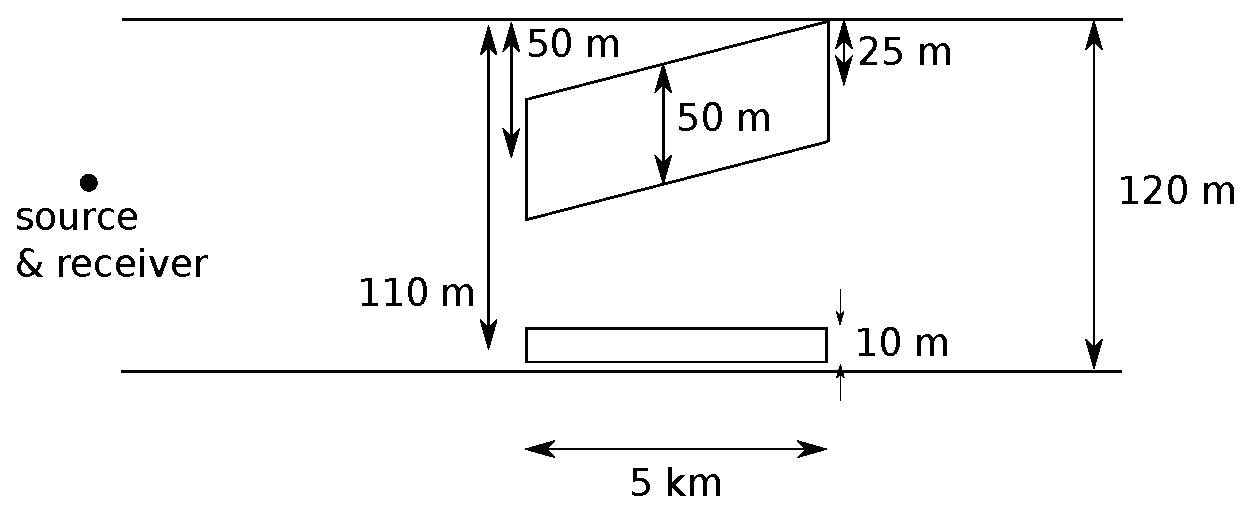
\includegraphics[width=0.8\textwidth]{{./figs/syntheticConfiguration20180515}.eps}}
  \caption{Range-depth configuration of the fish group}
  \label{fig:configSynthetic}
\end{figure}

\noindent Neutral buoyancy of the fish group is assumed to be 10 m below the sea surface and each vertical layer includes equal fish population.
Areal number density along the range within the fish group is shown in Fig. \ref{fig:naSynthetic}. 
The maximum areal number density is approximately 4.5 fish/m$^2$ at 2.5 km range.

\begin{figure}[htp!]
  \centering
  {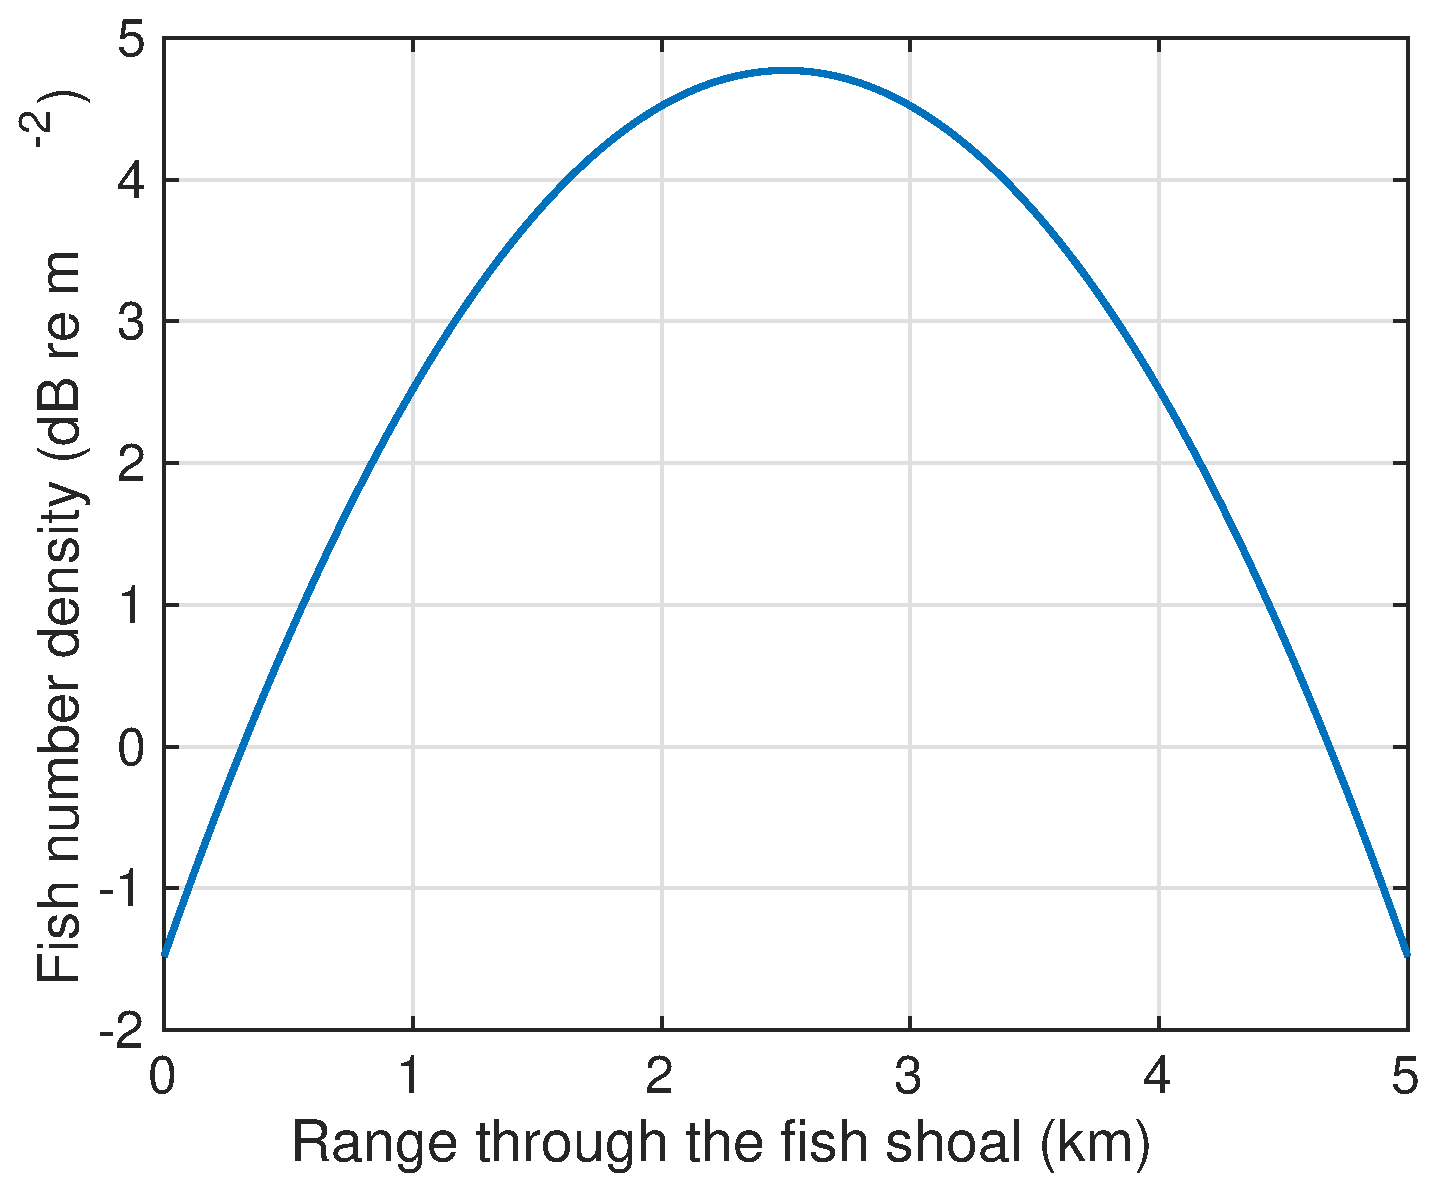
\includegraphics[width=0.5\textwidth]{{./figs/nASynthetic20180515}.eps}}
  \caption{Synthetic areal number density through the fish group}
  \label{fig:naSynthetic}
\end{figure}

\noindent Synthetic SS from this fish group is shown in Figs. \ref{fig:ssSyntheticWithNoise} and \ref{fig:ssSyntheticWithoutNoise}, where Fig. \ref{fig:ssSyntheticWithNoise} includes a zero-mean Gaussian white noise with 3 dB standard deviation and Fig. \ref{fig:ssSyntheticWithoutNoise} shows the SS without any noise.
SS at 1465 Hz and 1600 Hz are strong at close ranges but also shows the most attenuation as shown in Fig. \ref{fig:ssSyntheticWithoutNoise} because the resonance scattering frequency is near 1500 Hz as shown in Fig. \ref{fig:tsSynthetic}.

\begin{figure}[htp!]
  \centering
  {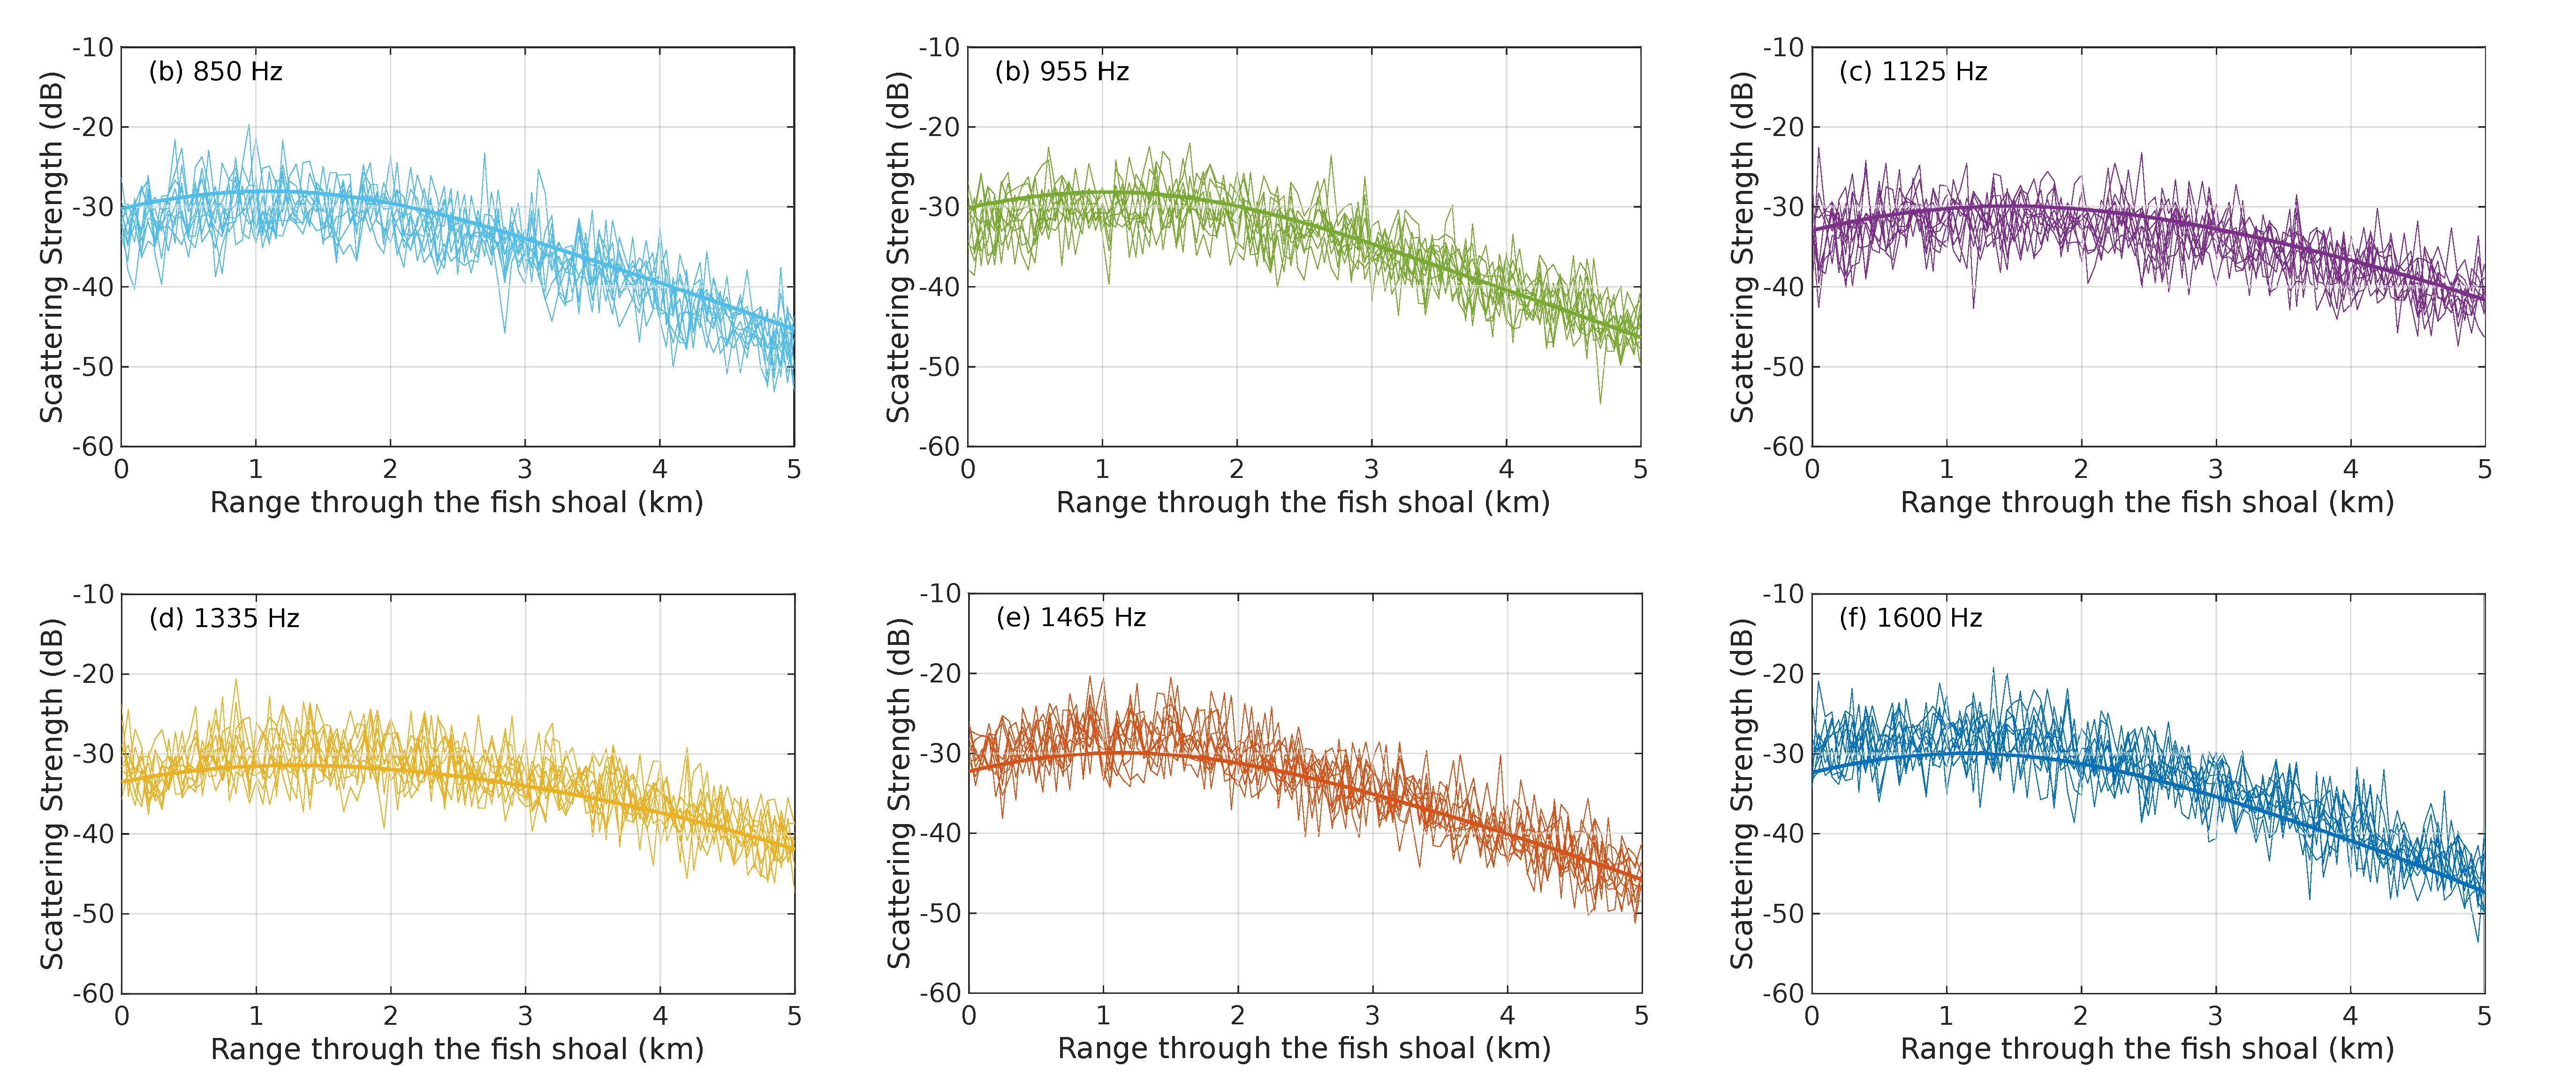
\includegraphics[width=1\textwidth]{{./figs/syntheticSSCombined_20180515}.eps}}
  \caption{Synthetic Scattering Strength (SS) through the fish group with zero-mean Gaussian white noise with 3 dB standard deviation. 10 SS curves are randomly realized at each frequency.}
  \label{fig:ssSyntheticWithNoise}
\end{figure}

\begin{figure}[htp!]
  \centering
  {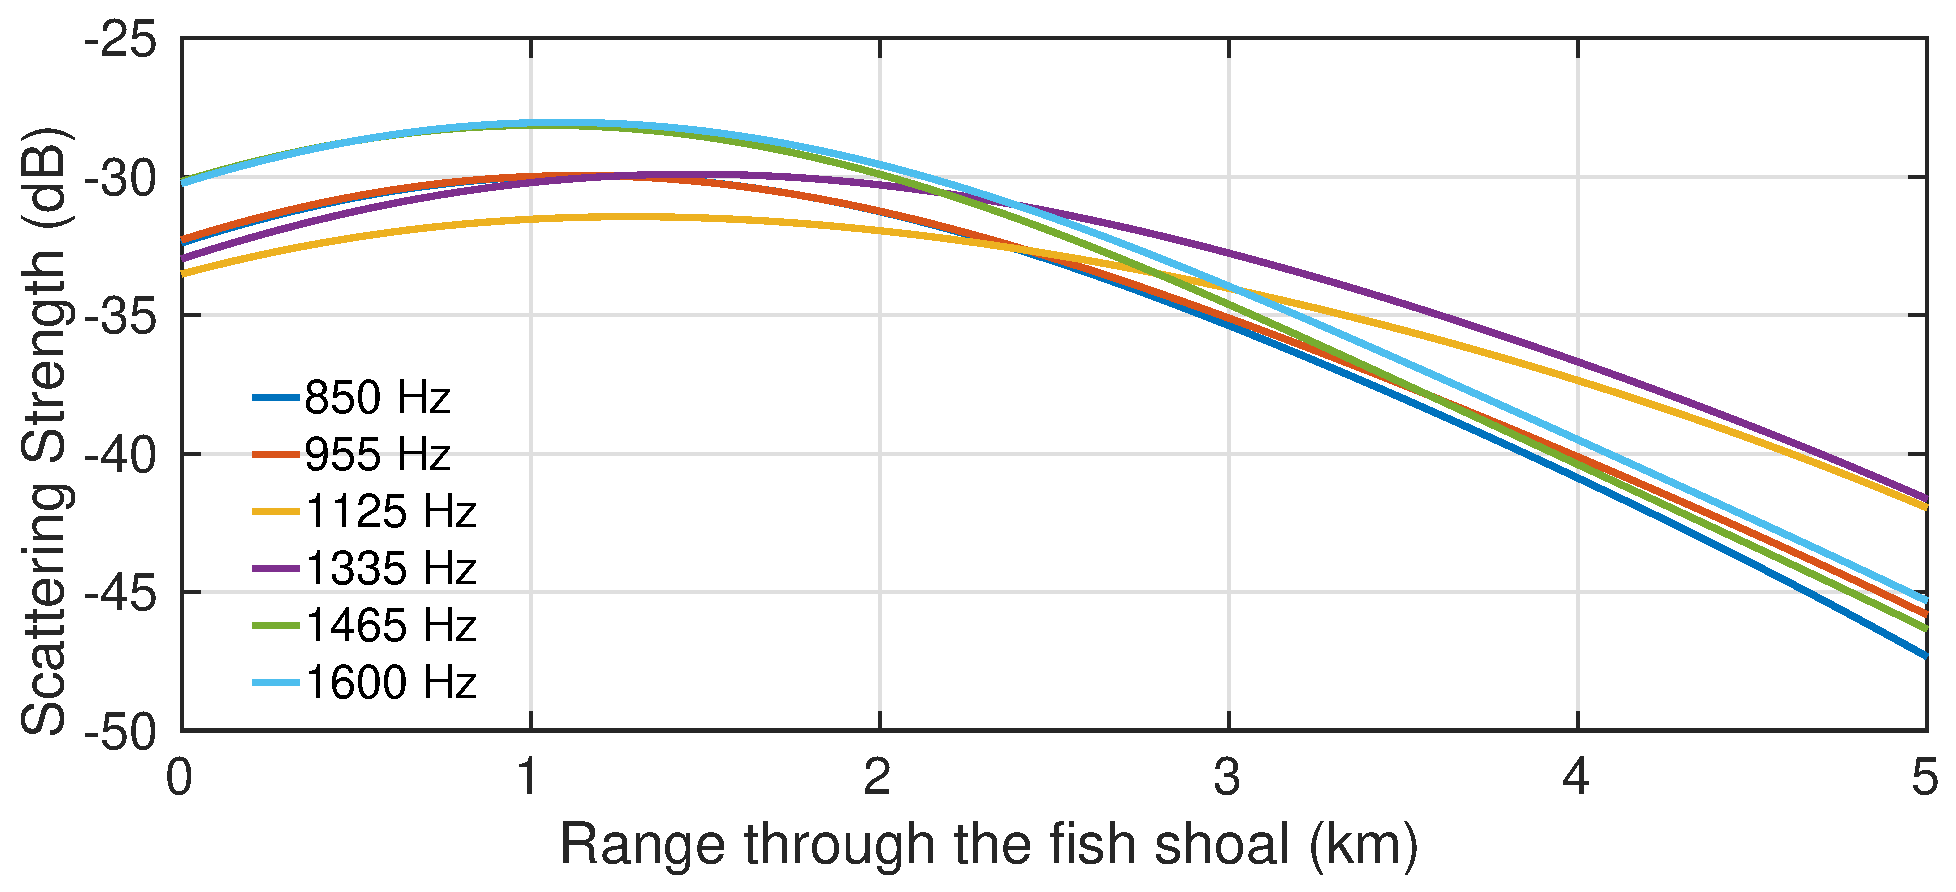
\includegraphics[width=0.6\textwidth]{{./figs/ssSynthetic20180515}.eps}}
  \caption{Synthetic Scattering Strength (SS) through the fish group without noise}
  \label{fig:ssSyntheticWithoutNoise}
\end{figure}

% \noindent SS at 850 and 1465 Hz are strongest at close ranges but also shows the most attenuation as shown in the Target Strength curve in Figure \ref{fig:tsSynthetic}.

\begin{figure}[htp!]
  \centering
  {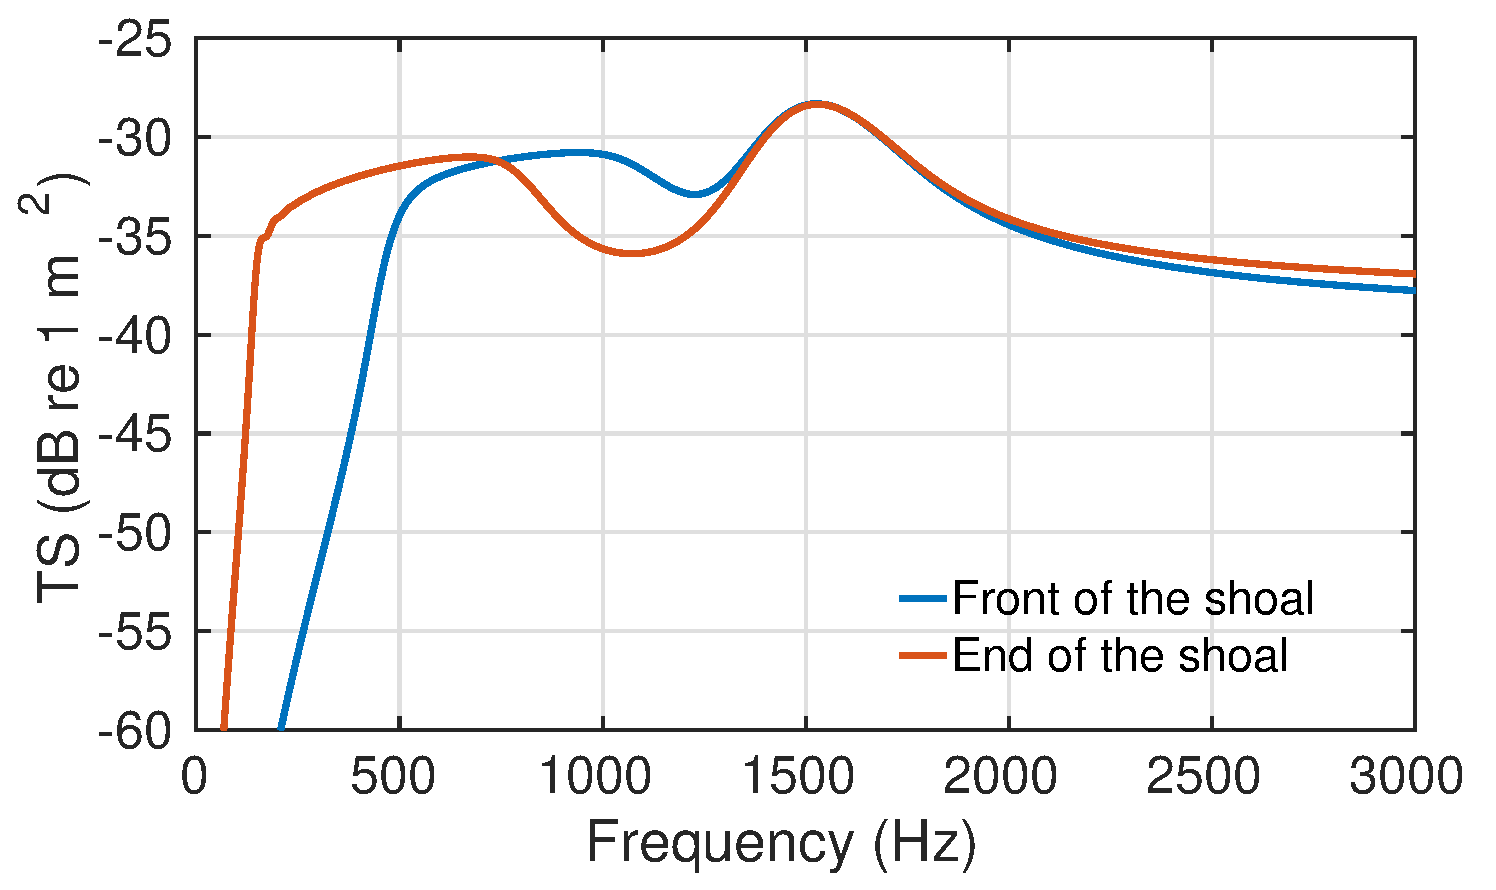
\includegraphics[width=0.5\textwidth]{{./figs/tsSynthetic20180515}.eps}}
  \caption{Synthetic Target Strength (TS) at the front and end of the group}
  \label{fig:tsSynthetic}
\end{figure}

EKF is applied to this synthetic SS data where 10 measurements at each range step are used to predict and update the state vector. 
The measurement noise covariance matrix $\boldsymbol{Q}_k$ is a diagonal matrix since each measurement is assumed uncorrelated and noise at each frequency is assumed uncorrelated. 
Small random perturbation is included in $\boldsymbol{Q}_k$ to resolve a singularity issue caused when multiple measurements following an identical distribution is used.
The process noise covariance matrix $\boldsymbol{R}_k$ is also a diagonal matrix since each state parameter is assumed uncorrelated with each other.


For a synthetic data set without any noise, Figs. \ref{fig:ekfEstimationWithoutNoise1} and \ref{fig:ekfEstimationWithoutNoise2} show the state estimate using the developed EKF.
In general, the estimation is better at closer range steps and deviates from the ground truth as the range steps increases.
EKF estimation of the fish vertical distribution is shown in Fig. \ref{fig:ekfEstimationWithoutNoise1}.
Mean occupancy depth estimation errors of the upper and lower fish layers (Fig. \ref{fig:ekfEstimationWithoutNoise1} (a) and (c)) are within 3 \% with respect to their ground truth vertical thicknesses.
Vertical thickness estimation error of the upper and lower fish layers (Fig. \ref{fig:ekfEstimationWithoutNoise1} (b) and (d)) are within 20 \% with respect to their ground truth vertical thicknesses.
EKF estimation of the fractional population of the upper fish layer, neutral buouancy depth and areal number density are accurate to be less than 1\% error with respect to their ground truth values.

\begin{figure}[htp!]
  \centering
  {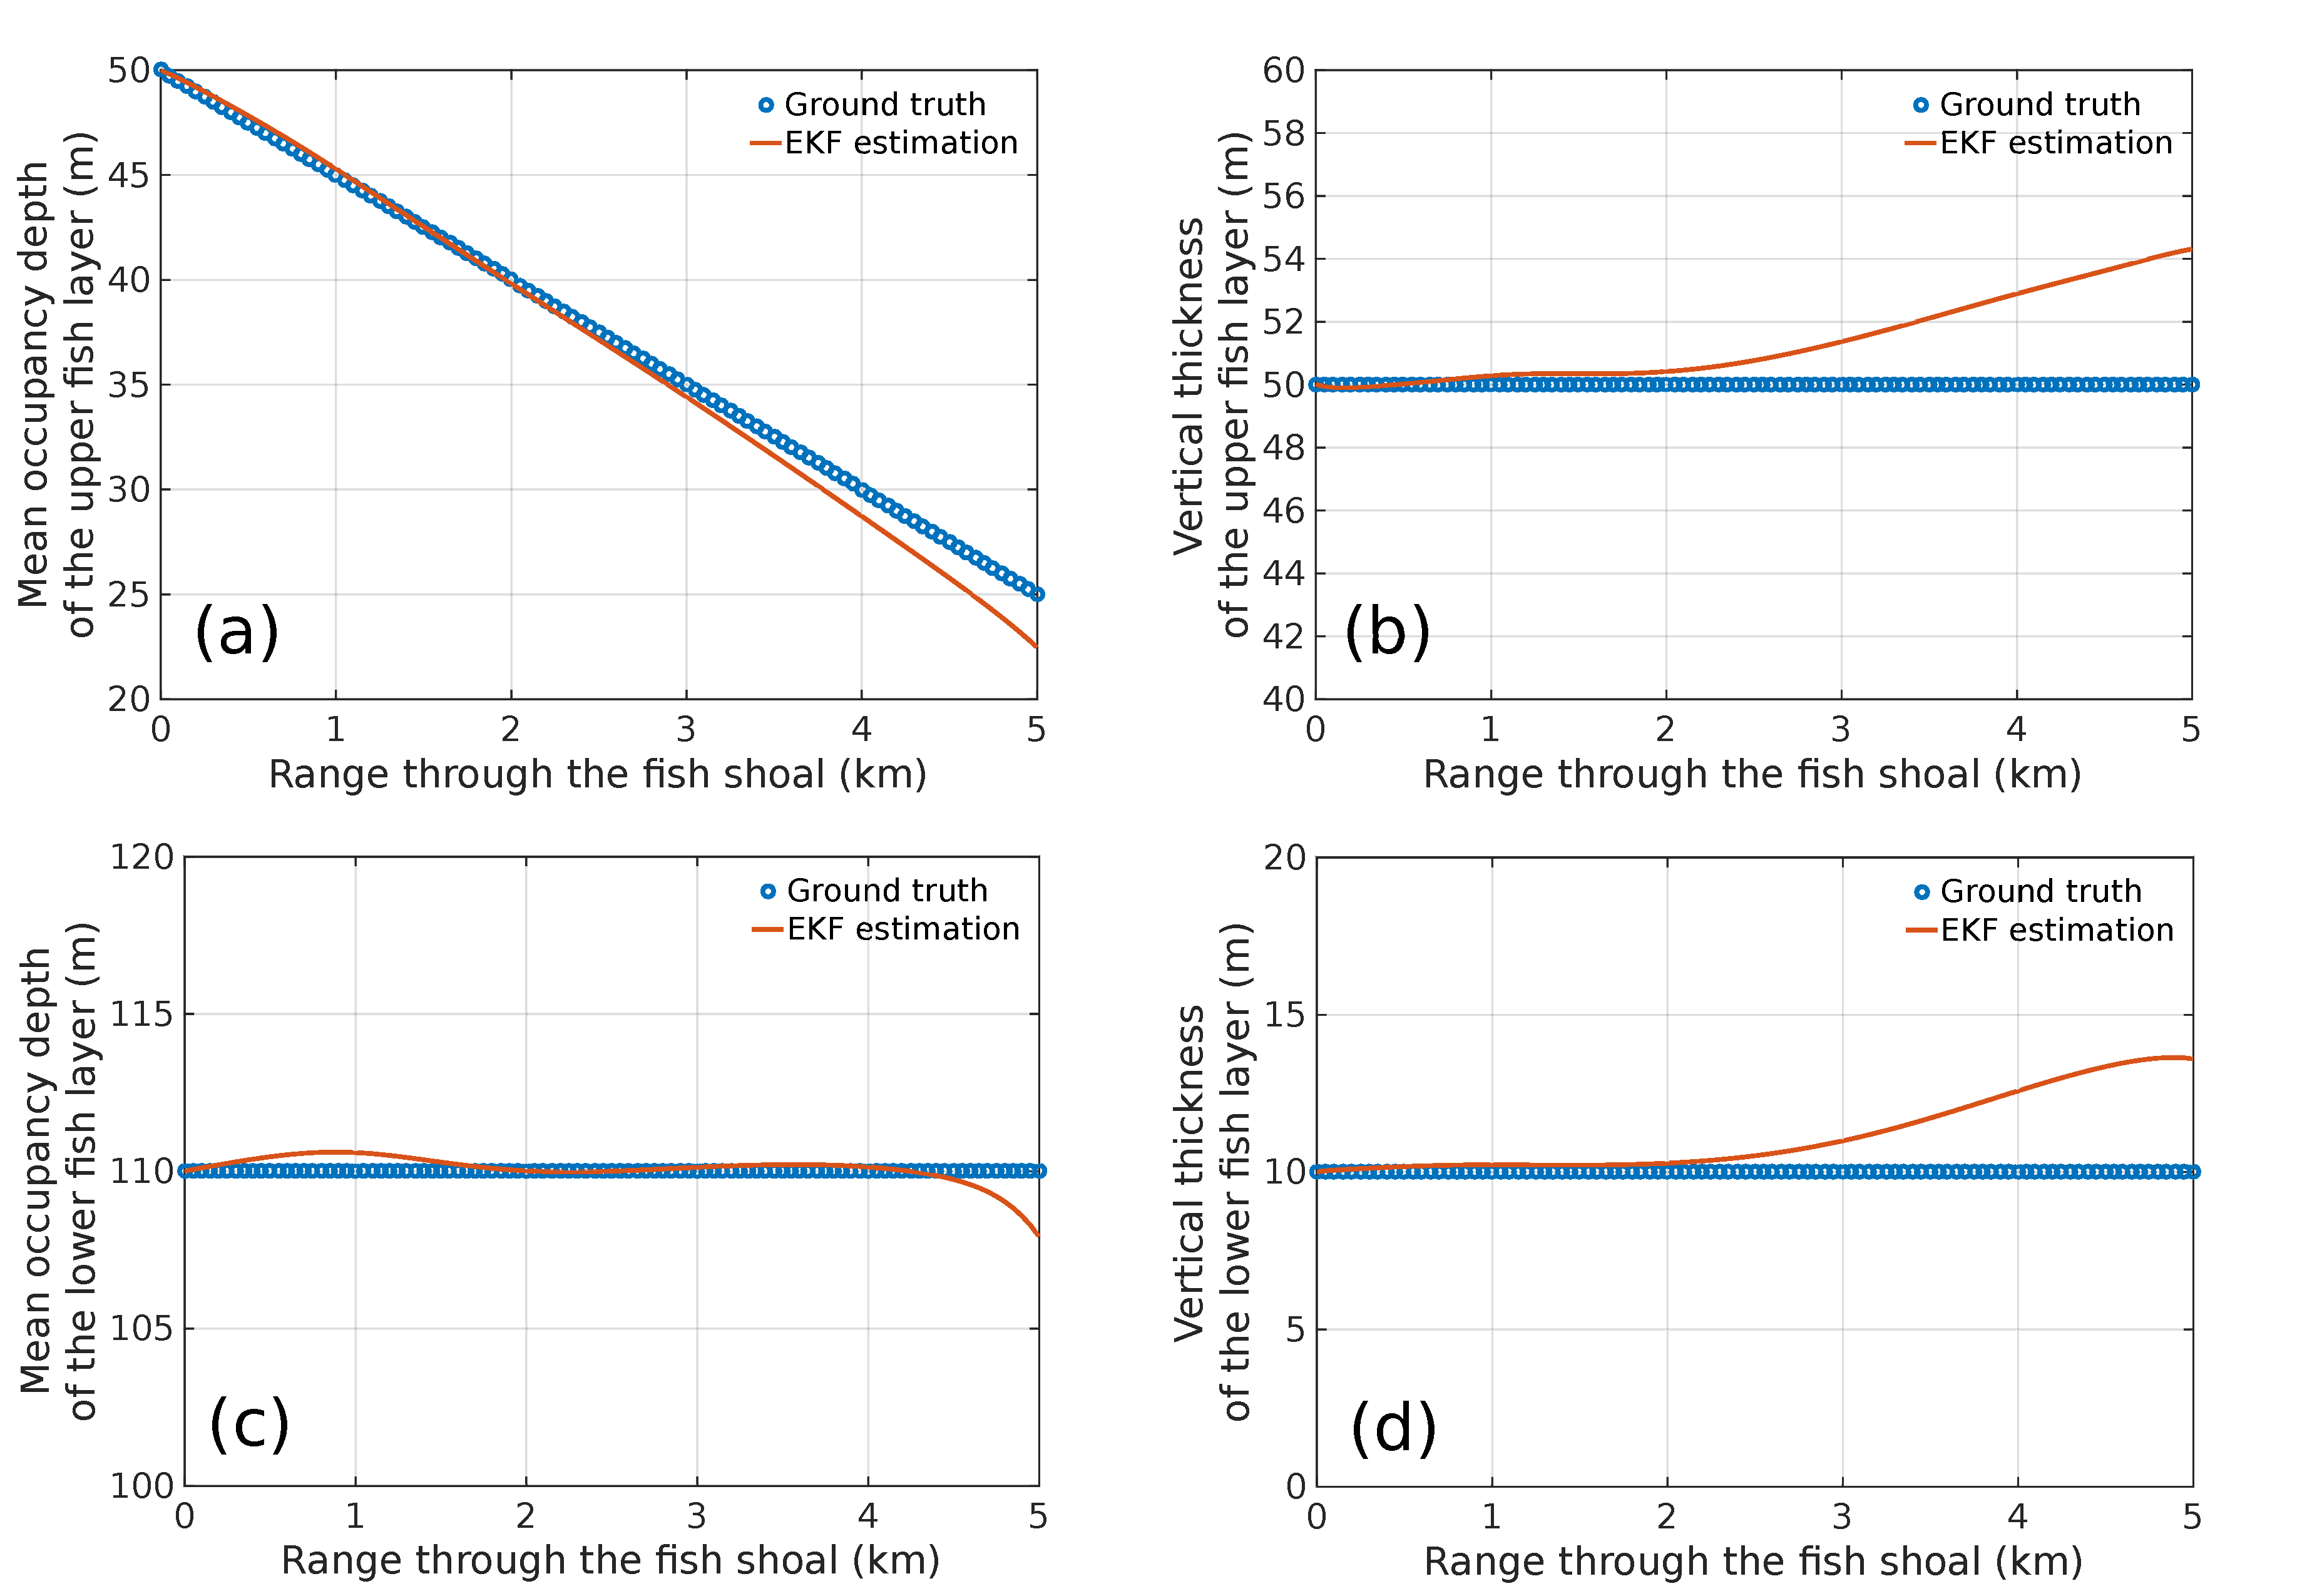
\includegraphics[width=0.8\textwidth]{{./figs/ekfEstimationWithoutNoiseH1_Z1_H2_Z2_20180515}.eps}}
  \caption{Extended Kalman Filter estimation of the fish depth distribution without any noise in the measurements.}
  \label{fig:ekfEstimationWithoutNoise1}
\end{figure}

\begin{figure}[htp!]
  \centering
  {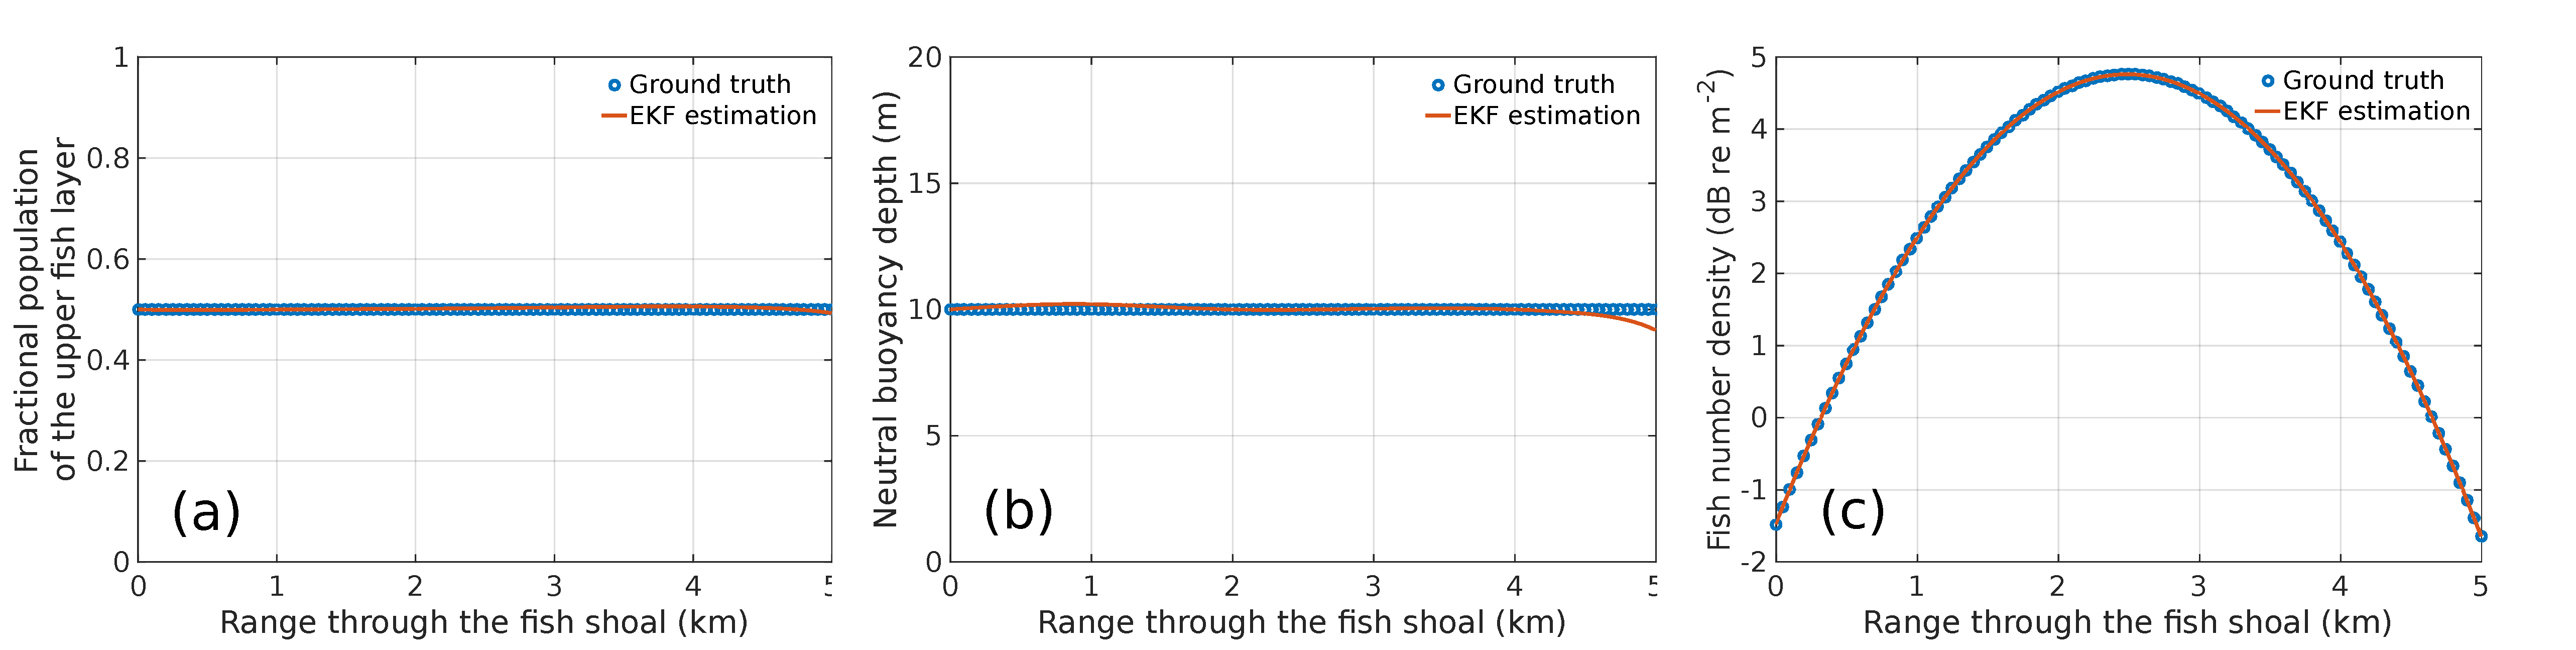
\includegraphics[width=1\textwidth]{{./figs/ekfEstimationWithoutNoiseRatio_Znb_nA_20180515}.eps}}
  \caption{Extended Kalman Filter estimation of (a) the fractional population of the upper fish layer, (b) neutral buoyancy depth and (c) areal number density without any noise in the measurements.}
  \label{fig:ekfEstimationWithoutNoise2}
\end{figure}

Similarly, EKF estimation results for synthetic measurements with noise are shown in Figs. \ref{fig:ekfEstimationWithNoise1} and \ref{fig:ekfEstimationWithNoise2}.
Mean occupancy depth estimation errors of the upper and lower fish layers (Fig. \ref{fig:ekfEstimationWithNoise1} (a) and (c)) are within 15 \% with respect to their ground truth vertical thicknesses.
Vertical thickness estimation errors of the upper and lower fish layers (Fig. \ref{fig:ekfEstimationWithoutNoise1} (b) and (d)) are within 25 \% with respect to their ground truth vertical thicknesses.
Estimation of the fractional population of the upper fish layer, neutral buouancy depth and areal number density are accurate to be less than 10\% error with respect to their ground truth values.





\begin{figure}[htp!]
  \centering
  {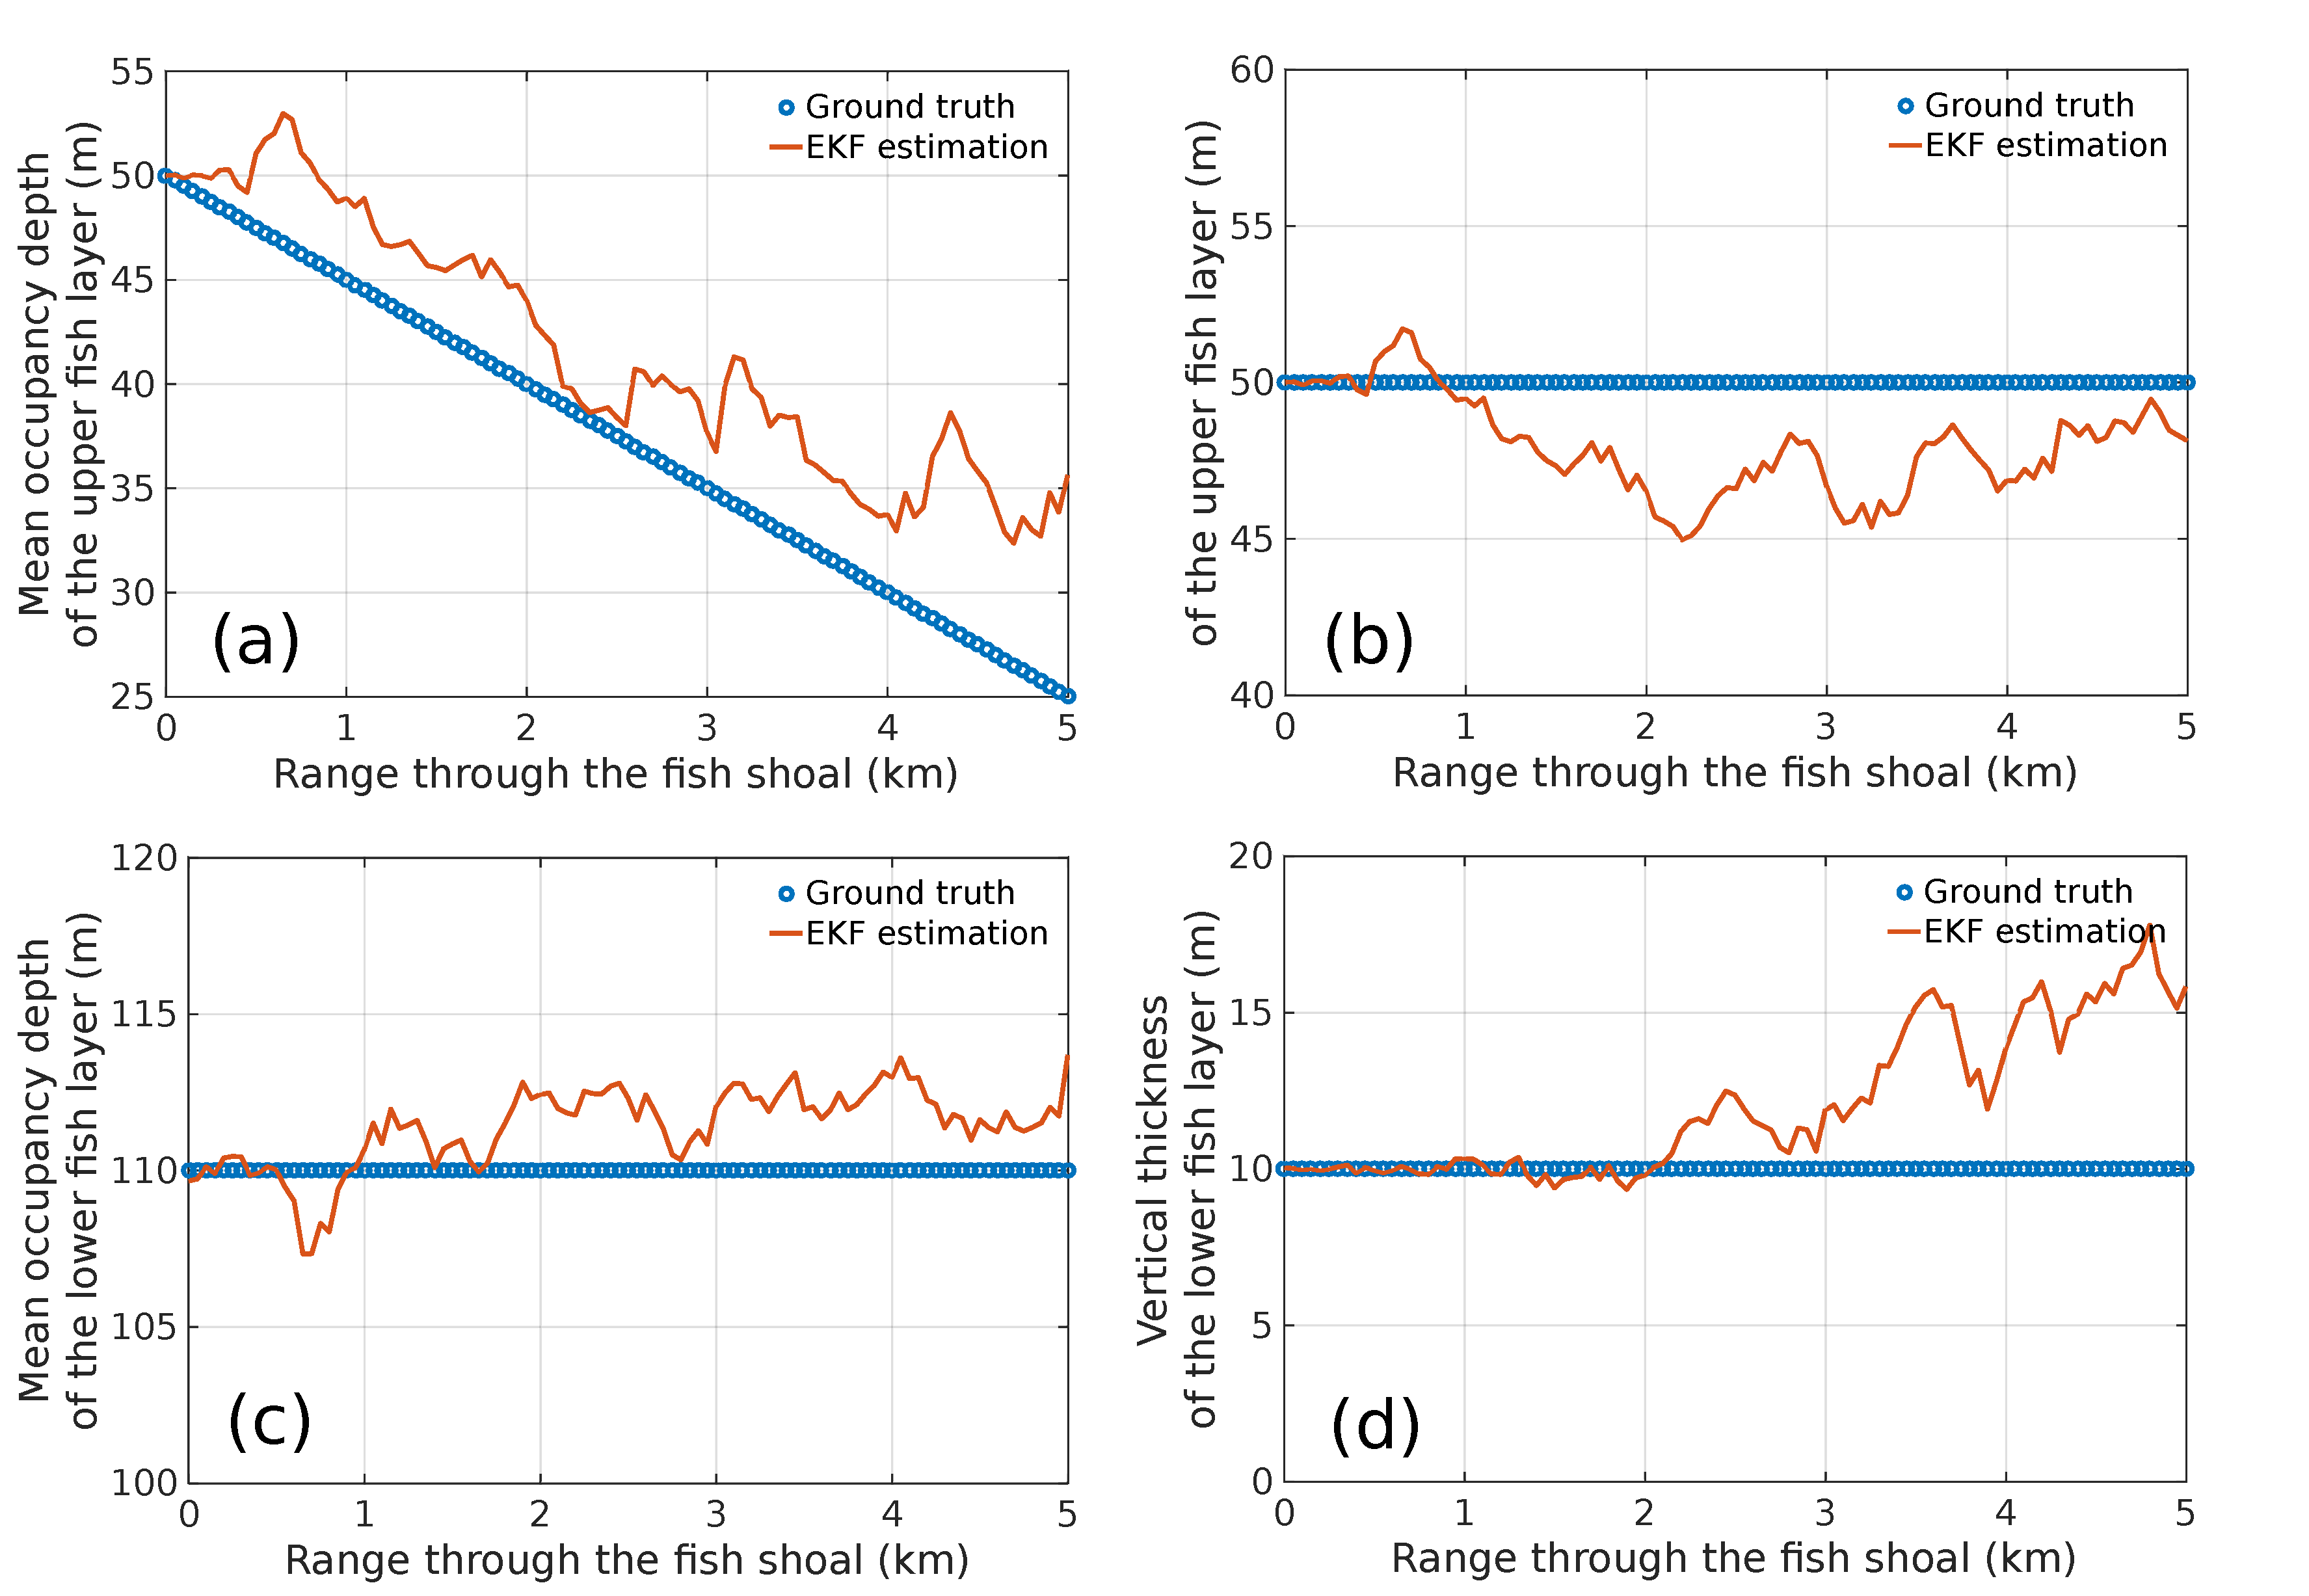
\includegraphics[width=0.8\textwidth]{{./figs/ekfEstimationWithNoiseZ1_H1_Z2_H2_20180515}.eps}}
  \caption{Extended Kalman Filter estimation of the fish depth distribution in the presence of zero-mean Gaussian white measurement noise with 3 dB standard deviation.}
  \label{fig:ekfEstimationWithNoise1}
\end{figure}

\begin{figure}[htp!]
  \centering
  {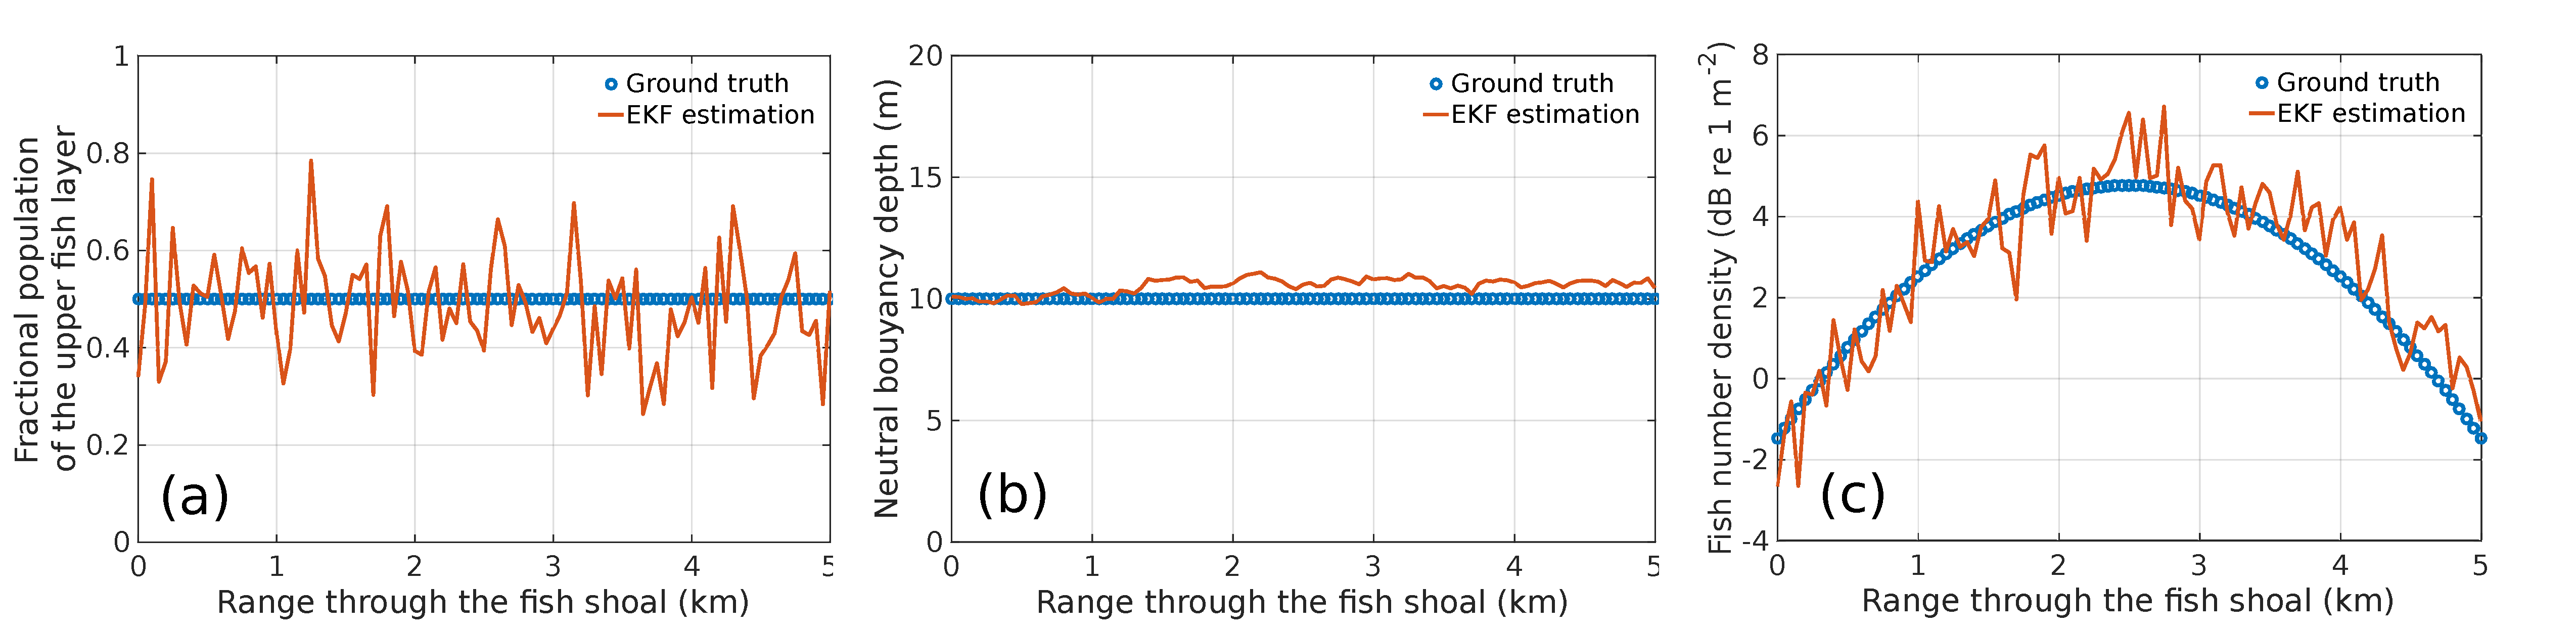
\includegraphics[width=1\textwidth]{{./figs/ekfEstimationWithNoiseRatio_Znb_nA_20180515}.eps}}
  \caption{Extended Kalman Filter estimation of (a) the fractional population of the upper fish layer, (b) neutral buoyancy depth and (c) areal number density in the presence of zero-mean Gaussian white measurement noise with 3 dB standard deviation.}
  \label{fig:ekfEstimationWithNoise2}
\end{figure}

\FloatBarrier

% \subsection{Temporal evolution of the frequency response of Coalescing Herring shoals}
% Multiple herring shoals coalesced during the night of Februrary 20th, 2014  over a 1.5 hour time period from 22:10:00 to 23:20:00 UTC in the northwest region of the trench near Alesund. 
% Bathymetry of this region is shown in Fig. \ref{fig:bathymetry}.

% \begin{figure}[htp!]
%   \centering
%   {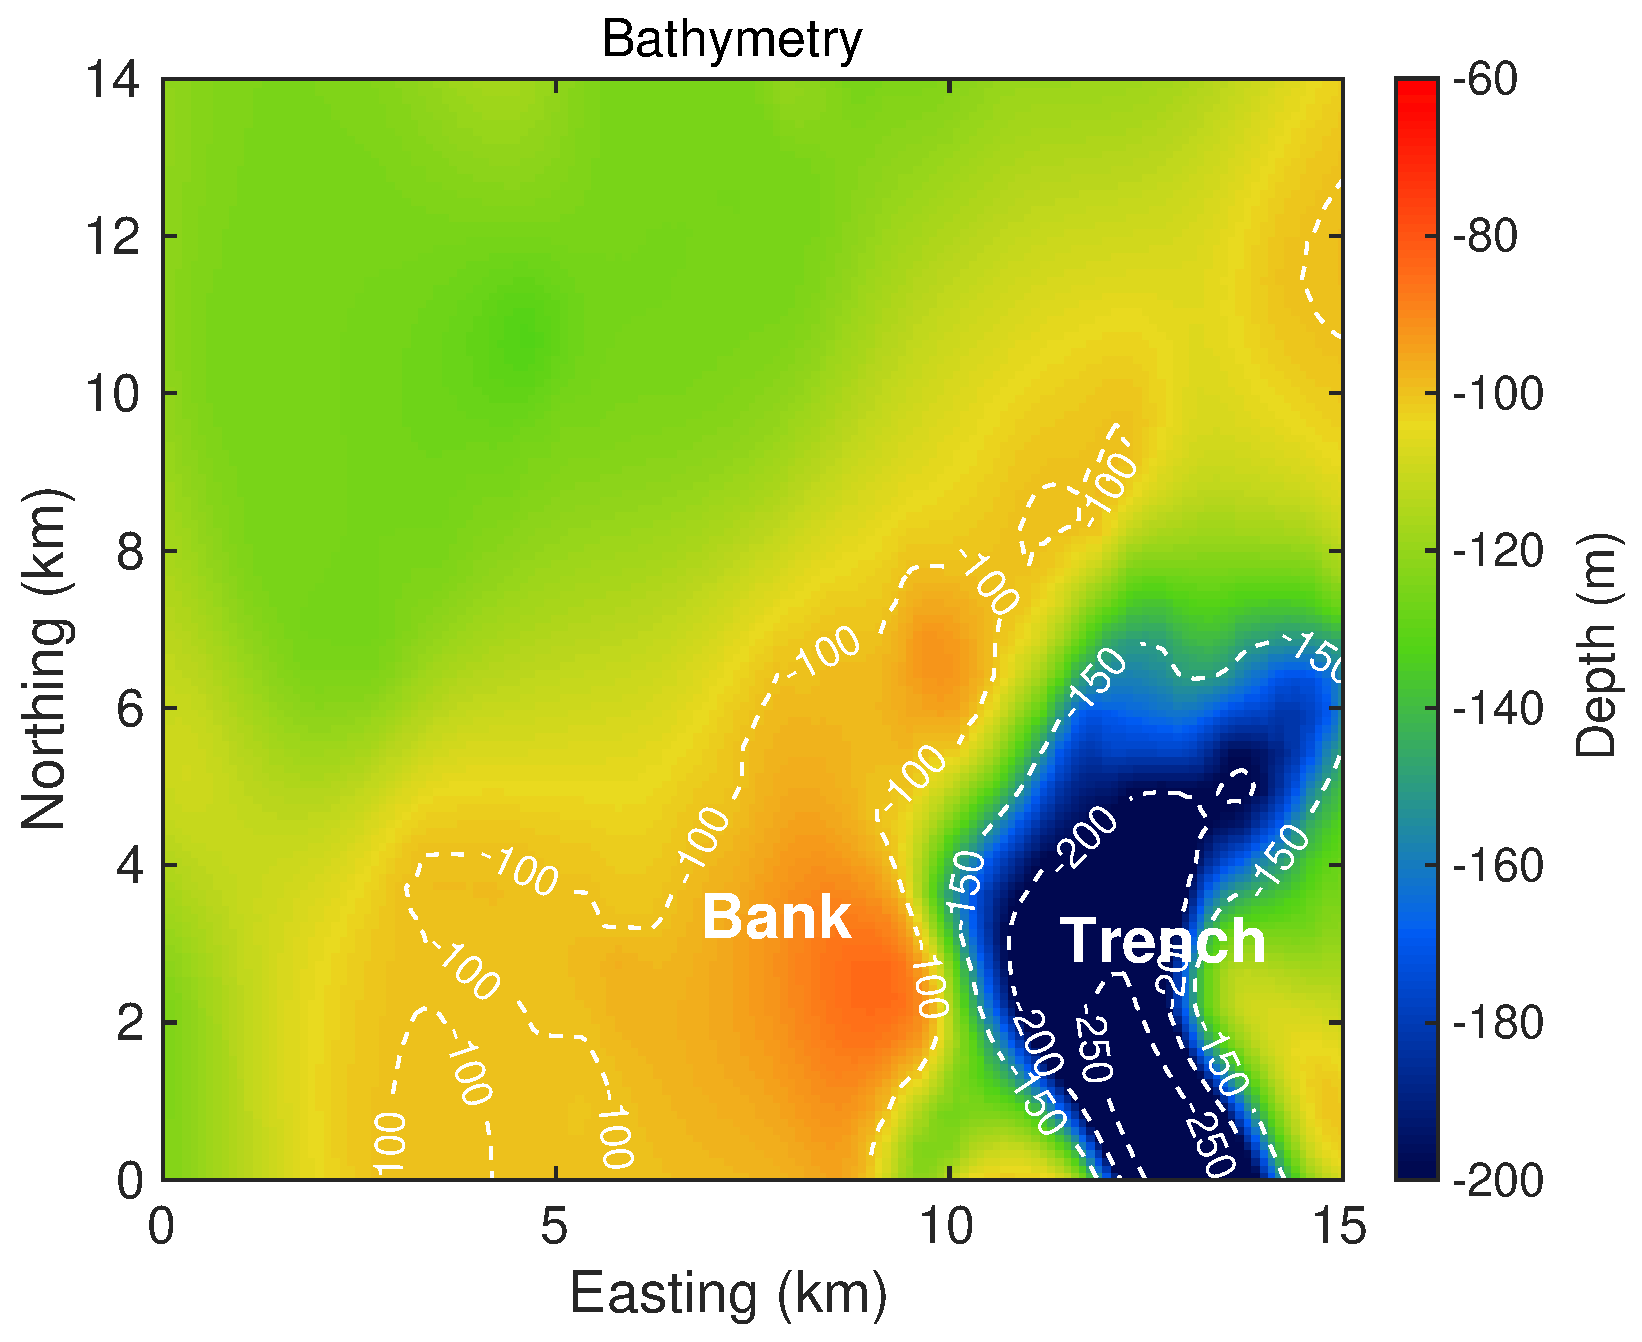
\includegraphics[width=0.7\textwidth]{{./figs/bathyMap}.eps}}
%   \caption{
%   Bathymetry near the northwest region of the trench near Alesund, Norway.
%   }
%   \label{fig:bathymetry}
% \end{figure}


% At the beginning of the track, near 22:00:00, RV Knorr heads southwest and the shoals distributed in the southeastern region of the ship starts to coalesce. 
% The ship slowly turns it’s heading to south while the coalescing shoals on the left to the ship heading are monitored throughout the track. The shoals coalesce towards the northern flank of the bank where the water depth gradually changes from 120 m to 100 m.
% Resonant acoustic scattering frequency of these multiple coalescing shoals is found to be between 850 Hz and 955 Hz during the migration, then shifts towards 1125 Hz after the shoals merge into a larger single shoal.
% After the shoals merge into a larger shoal, frequency response of the dense shoal region peaks at 955 Hz, whereas that of the diffuse shoal region peaks at 1125 Hz. 
% This implies the fish in the dense shoal region occupies a shallower water depth than those in the diffuse shoal region given a constant neutral buoyancy depth.

% Temporal evolution of the frequency response of multiple coalescing shoals is analyzed. 
% the shoal boundary indicated by the black contour lines is determined by scaling down the Herring shoal critical density found in the Gulf of Maine, 0.2 fish/m$^2$, by the body length ratio squared, and using a calibrated mean Target Strength (TS) at 955 Hz ($\overline{\text{TS}}_\text{955 Hz} = -30 $ dB re 1 m$^2$) near this region.
% The magenta contour lines indicate the dense shoal region where the SS levels are 6 dB higher than that of the black contour lines.
% To reduce the variance, pings within 5 minute time window are averaged at each frequency. At 955 Hz, 6 consecutive pings are available within the 5 minute time window, whereas at the other frequencies, 850, 1125, 1335, 1465 and 1600 Hz, 2 consecutive pings are available. 
% % Figure 1(b), (c) and (d) show the Scattering Strength (SS) maps at 955 Hz at the three time windows chosen for the analysis. 
% Figs. \ref{fig:evolutionShoal1}, \ref{fig:evolutionShoal2}, \ref{fig:evolutionShoal3} and \ref{fig:evolutionShoal4} show the frequency response evolution over time before they form a large shoal (roughly, 22:10:00 to 23:10:00 UTC).
% Portion of the shoal shown in Fig. \ref{fig:evolutionShoal1}(a) migrates towards south, merging with other shoals to form a larger shoal.
% The other portion of this shoal splits into small schools and scatter, moving roughly towards the northeast direction.
% Peak of the frequency response of this shoal gradually changes from near 955 Hz to 1125 Hz as this shoal migrates southwards.
% % When the ship turns, the SS levels are not stable because the receiver array does not remain straight. 
% % Pings during the time windows within which the ship is not turning or zigzagging are used for the frequency response analysis. 
% Another shoal that is shown in Fig. \ref{fig:evolutionShoal2} starts to form at around 22:20:00 UTC.
% This shoal develops over roughly an hour period and merges with other shoals to form a single large shoal.
% During this shoal formation and colaescence, peak of the frequency response gradually changes from near 955 Hz to 1125 Hz.
% The shoal in Fig. \ref{fig:evolutionShoal3} shows a similar frequency response evolution with the shoals in Figs. \ref{fig:evolutionShoal1} and \ref{fig:evolutionShoal2} over the same time period.
% As this shoal develops and merges with other shoals, peak of the frequency response gradually changes from near 955 Hz to 1125 Hz. 
% Coalescence of the largest migrating shoal is shown in Fig. \ref{fig:evolutionShoal4}.
% This shoal migrates southwest towards the northern tip of the bank.
% During the migration, peak of the frequency response remains stable near and below 955 Hz.
% Fig. \ref{fig:evolutionShoalMerged} shows the frequency response after the 4 shoals (either formed or migrated) merged together.
% The resonant peak frequency is near 1125 Hz, where the peak is more apparent for the diffuse region of the shoal.
% For the denser region of the shoal, the resonance peak frequency is below 1125 Hz. 
% This implies that the fish in the dense shoal region occupies a shallower water depth than those in the diffuse shoal region.

% % Figure 2(a) and (b) show the frequency responses when the shoal is migrating and Figure 2(c) shows the frequency response when the shoal is relatively stationary near the northern flank of the bank. The black solid lines indicate the frequency responses of the entire shoal within the black contours of the SS maps in Figure 1. The magenta solid lines show the frequency responses of the dense shoal region within the magenta contours of the SS maps and the blue solid lines show the frequency responses of the diffuse shoal region between the black and magenta contours of the SS maps.
% % In Figure 2(a), showing the frequency response when the shoal starts to migrate, the resonance frequency is below or near 850 Hz and the frequency response patterns of the dense and diffuse shoal region are similar. In Figure 2(b), the shoal migrates towards the northern flank of the bank and shows the resonance frequency shift towards 955 Hz. The resonance peak at 955 Hz is sharper in the dense shoal region than that in the diffuse shoal region. In Figure 2(c), the shoal arrives at the northern flank of the bank and remains relatively stationary. The resonance frequency shifts to 1125 Hz for the entire shoal, however the resonance frequencies of the dense and diffuse shoal regions are different. While the resonance frequency of the dense shoal region is 955 Hz, that of the diffuse shoal region is 1125 Hz. Given a constant neutral buoyancy depth, this implies the fish in the dense shoal region occupies a shallower water depth than those in the diffuse shoal region.

% \begin{figure}[H]
%   \centering
%   \subfigure
%   	{\includegraphics[height=0.3\textwidth]{{figs/shoal1/ssMap20140220221354f0955Hz}.eps}}
%   \subfigure
%   	{\includegraphics[height=0.3\textwidth]{{figs/shoal1/freqResponse20140220221149_221559}.eps}}
% 	\\ \vspace{-10pt}
%   \subfigure
%   	{\includegraphics[height=0.3\textwidth]{{figs/shoal1/ssMap20140220223354f0955Hz}.eps}}
%   \subfigure
%   	{\includegraphics[height=0.3\textwidth]{{figs/shoal1/freqResponse20140220223149_223559}.eps}}
%   \\ \vspace{-10pt}
% 	\subfigure
%   	{\includegraphics[height=0.3\textwidth]{{figs/shoal1/ssMap20140220224444f0955Hz}.eps}}
% 	\subfigure
%   	{\includegraphics[height=0.3\textwidth]{{figs/shoal1/freqResponse20140220224239_224649}.eps}}
%   \\ \vspace{-10pt}
%   \subfigure
%   	{\includegraphics[height=0.3\textwidth]{{figs/shoal1/ssMap20140220225444f0955Hz}.eps}}
%   \subfigure
%   	{\includegraphics[height=0.3\textwidth]{{figs/shoal1/freqResponse20140220225239_225649}.eps}}
%   \\ \vspace{-10pt}
%   \subfigure
%   	{\includegraphics[height=0.3\textwidth]{{figs/shoal1/ssMap20140220230444f0955Hz}.eps}}
%   \subfigure
%   	{\includegraphics[height=0.3\textwidth]{{figs/shoal1/freqResponse20140220230239_230649}.eps}}
% 	\caption{
% 	Frequency response evolution of one of the coalescing herring shoals from rougly 22:10:00 to 23:05:00 UTC on February 20, 2014 near Alesund, Norway.
% 	While this shoal migrates towards south, part of the shoal merges with other shoals and form a larger shoal.
% 	The other portion of the initial shoal splits into multiple small schools and scatter.
% 	Peak of the frequency response of this shoal gradually changes from near 955 Hz to 1125 Hz.}
%   \label{fig:evolutionShoal1}
% \end{figure}

% \begin{figure}[H]
%   \centering
%   \subfigure
%   	{\includegraphics[height=0.3\textwidth]{{figs/shoal2/ssMap20140220222304f0955Hz}.eps}}
%   \subfigure
%   	{\includegraphics[height=0.3\textwidth]{{figs/shoal2/freqResponse20140220222059_222509}.eps}}
% 	\\ \vspace{-10pt}
%   \subfigure
%   	{\includegraphics[height=0.3\textwidth]{{figs/shoal2/ssMap20140220225444f0955Hz}.eps}}
%   \subfigure
%   	{\includegraphics[height=0.3\textwidth]{{figs/shoal2/freqResponse20140220225239_225649}.eps}}
%   \\ \vspace{-10pt}
% 	\subfigure
%   	{\includegraphics[height=0.3\textwidth]{{figs/shoal2/ssMap20140220230444f0955Hz}.eps}}
% 	\subfigure
%   	{\includegraphics[height=0.3\textwidth]{{figs/shoal2/freqResponse20140220230239_230649}.eps}}
% 	\caption{
% 	Frequency response evolution of a herring shoal while it forms and coalesce with other shoals.
% 	This shoal starts to form at 22:20:00 UTC, February 20, 2014 and merges with multiple shoals.
% 	Peak of the frequency response of this shoal gradually changes from near 955 Hz to 1125 Hz.
% 	}
%   \label{fig:evolutionShoal2}
% \end{figure}

% \begin{figure}[H]
%   \centering
%   \subfigure
%   	{\includegraphics[height=0.3\textwidth]{{figs/shoal3/ssMap20140220222304f0955Hz}.eps}}
%   \subfigure
%   	{\includegraphics[height=0.3\textwidth]{{figs/shoal3/freqResponse20140220222059_222509}.eps}}
% 	\\ \vspace{-10pt}
%   \subfigure
%   	{\includegraphics[height=0.3\textwidth]{{figs/shoal3/ssMap20140220224444f0955Hz}.eps}}
%   \subfigure
%   	{\includegraphics[height=0.3\textwidth]{{figs/shoal3/freqResponse20140220224239_224649}.eps}}
%   \\ \vspace{-10pt}
% 	\subfigure
%   	{\includegraphics[height=0.3\textwidth]{{figs/shoal3/ssMap20140220225444f0955Hz}.eps}}
% 	\subfigure
%   	{\includegraphics[height=0.3\textwidth]{{figs/shoal3/freqResponse20140220225239_225649}.eps}}
% 	\\ \vspace{-10pt}
%   \subfigure
%   	{\includegraphics[height=0.3\textwidth]{{figs/shoal3/ssMap20140220230444f0955Hz}.eps}}
% 	\subfigure
%   	{\includegraphics[height=0.3\textwidth]{{figs/shoal3/freqResponse20140220230239_230649}.eps}}
% 	\caption{
% 	Frequency response evolution of one of the coalescing herring shoals.
% 	This shoal develops to a larger shoal and merges with multiple shoals and form a larger shoal.
% 	Peak of the frequency response of this shoal gradually changes from near 955 Hz to 1125 Hz.
% 	}
%   \label{fig:evolutionShoal3}
% \end{figure}


% \begin{figure}[H]
%   \centering
%   \subfigure
%   	{\includegraphics[height=0.3\textwidth]{{figs/shoal4/ssMap20140220222304f0955Hz}.eps}}
%   \subfigure
%   	{\includegraphics[height=0.3\textwidth]{{figs/shoal4/freqResponse20140220222059_222509}.eps}}
% 	\\ \vspace{-10pt}
%   \subfigure
%   	{\includegraphics[height=0.3\textwidth]{{figs/shoal4/ssMap20140220223354f0955Hz}.eps}}
%   \subfigure
%   	{\includegraphics[height=0.3\textwidth]{{figs/shoal4/freqResponse20140220223149_223559}.eps}}
%   \\ \vspace{-10pt}
% 	\subfigure
%   	{\includegraphics[height=0.3\textwidth]{{figs/shoal4/ssMap20140220225444f0955Hz}.eps}}
% 	\subfigure
%   	{\includegraphics[height=0.3\textwidth]{{figs/shoal4/freqResponse20140220225239_225649}.eps}}
% 	\\ \vspace{-10pt}
%   \subfigure
%   	{\includegraphics[height=0.3\textwidth]{{figs/shoal4/ssMap20140220230444f0955Hz}.eps}}
% 	\subfigure
%   	{\includegraphics[height=0.3\textwidth]{{figs/shoal4/freqResponse20140220230239_230649}.eps}}
% 	\caption{
% 	Frequency response evolution of one of the coalescing herring shoals.
% 	This shoal migrates southwest towards the bank and merges with multiple shoals and form a larger shoal.
% 	Peak of the frequency respone of this shoal remains near and below 955 Hz during the migration.
% 	% Peak of the frequency response of this shoal gradually changes from near 955 Hz to 1125 Hz.
% 	}
%   \label{fig:evolutionShoal4}
% \end{figure}

% \begin{figure}[H]
%   \centering
%   \subfigure
%   	{\includegraphics[height=0.3\textwidth]{{figs/shoalMerged/ssMap20140220231854f0955Hz}.eps}}
%   \subfigure
%   	{\includegraphics[height=0.3\textwidth]{{figs/shoalMerged/freqResponse20140220231649_232059}.eps}}
% 	\\ \vspace{-10pt}
%   \subfigure
%   	{\includegraphics[height=0.3\textwidth]{{figs/shoalMerged/ssMap20140220232854f0955Hz}.eps}}
%   \subfigure
%   	{\includegraphics[height=0.3\textwidth]{{figs/shoal4/freqResponse20140220232649_233059}.eps}}
% 	\caption{
% 	Frequency response evolution of the merged herring shoal.
% 	Peak of the frequency response of this merged shoal is 1125 Hz.
% 	}
%   \label{fig:evolutionShoalMerged}
% \end{figure}

% \begin{figure}[H]
%   \centering
%   \subfigure
%   	{\includegraphics[height=0.3\textwidth]{{figs/echogram}.png}}
% 	\\ \vspace{-10pt}
%   \subfigure
%   	{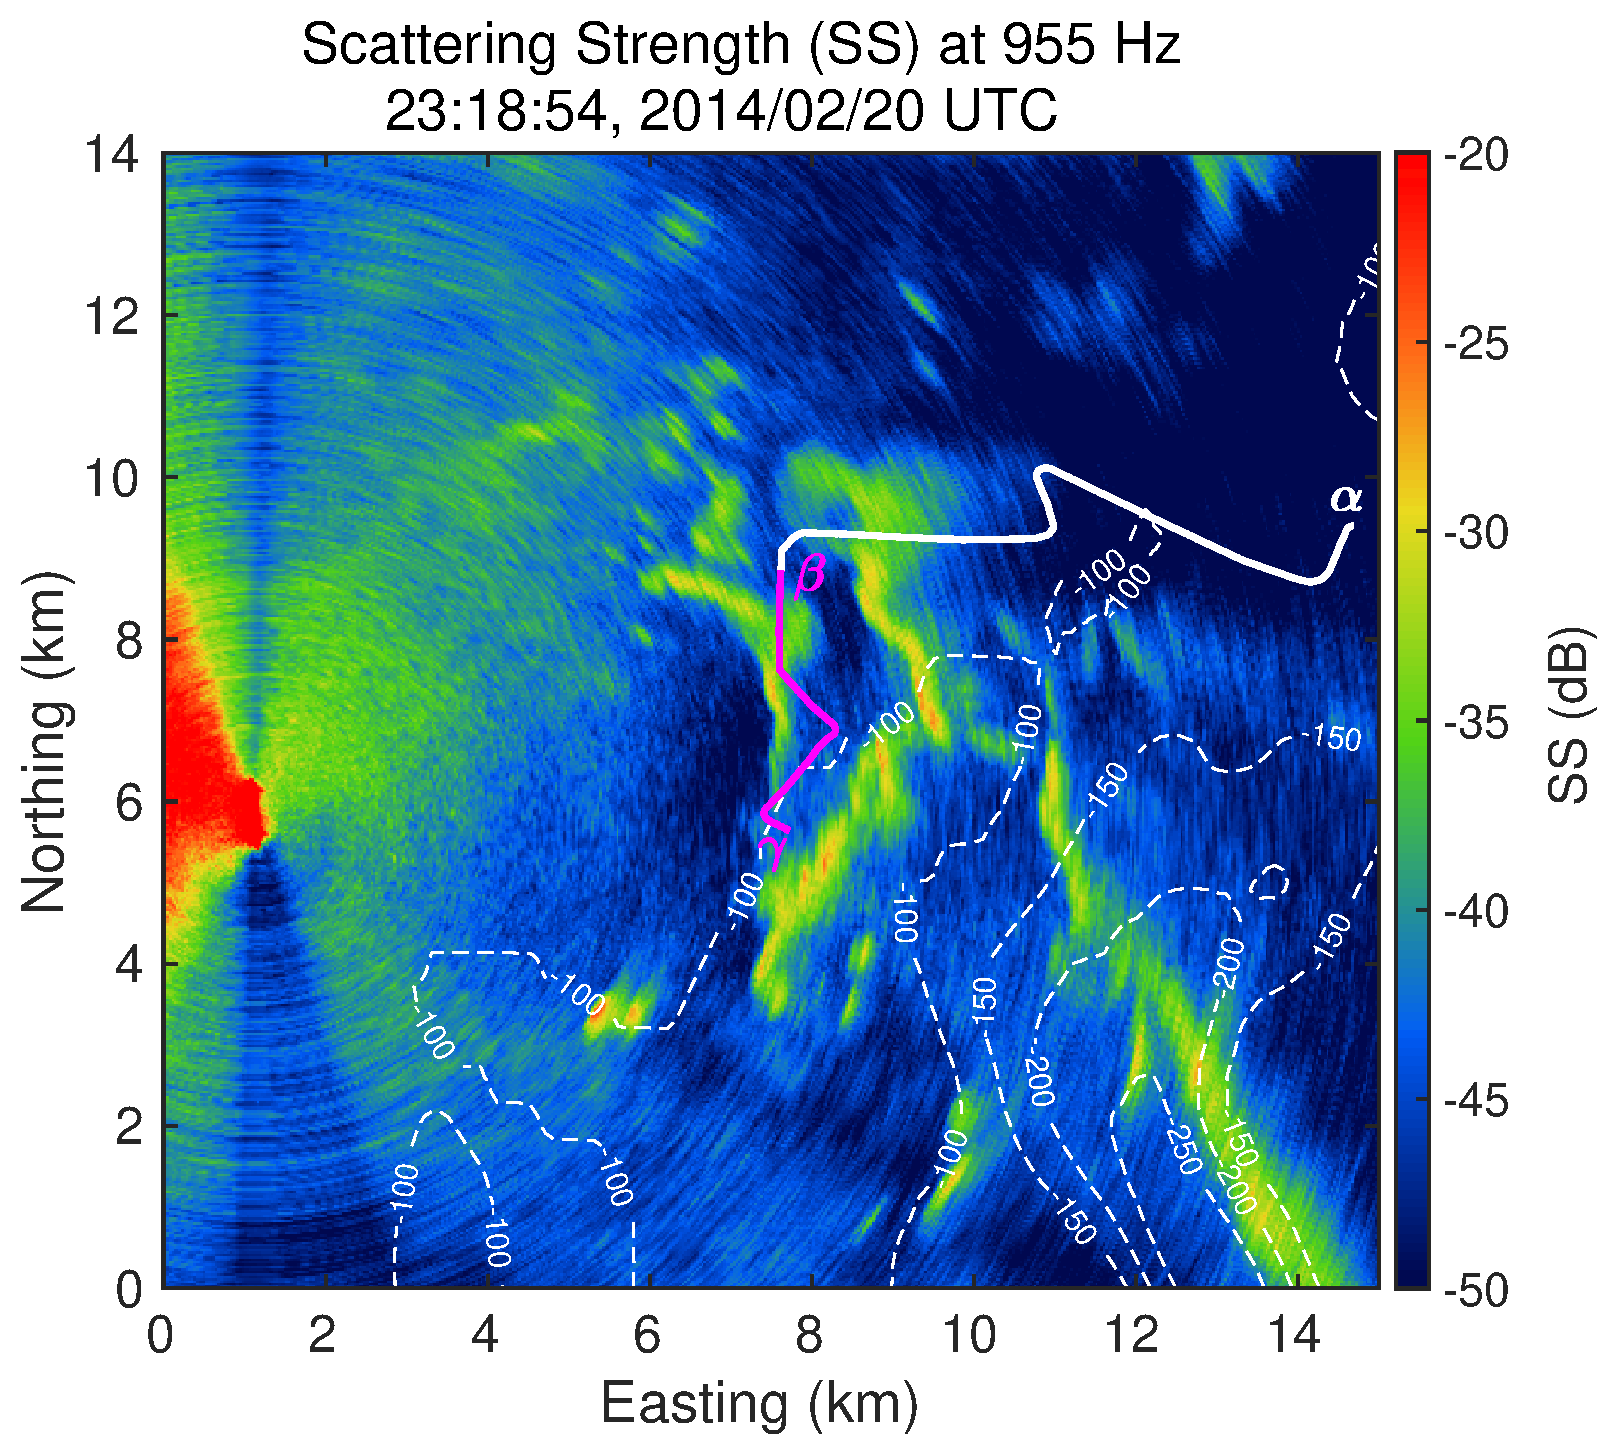
\includegraphics[height=0.6\textwidth]{{figs/echogramCorrespondance}.eps}}
% 	\caption{
% 	Echogram of the merged shoal.
% 	The echogram was taken an hour after the time when OAWRS image was taken.
% 	The meah shoal depth increases as the echogram ship moves into the shoal. 
% 	}
%   \label{fig:echogramConfirmation}
% \end{figure}


%%%%%%%%%%%%%%%%%%%%%%%%%%%%%%%%%%%%%%%%%%
\reftitle{References}
% \begin{thebibliography}{999}
% % Reference 1
% \bibitem[Author1(year)]{ref-journal}
% Author1, T. The title of the cited article. {\em Journal Abbreviation} {\bf 2008}, {\em 10}, 142-149, DOI.
% % Reference 2
% \bibitem[Author2(year)]{ref-book}
% Author2, L. The title of the cited contribution. In {\em The Book Title}; Editor1, F., Editor2, A., Eds.; Publishing House: City, Country, 2007; pp. 32-58, ISBN.
% \end{thebibliography}

% The following MDPI journals use author-date citation: Arts, Econometrics, Economies, Genealogy, Humanities, IJFS, JRFM, Laws, Religions, Risks, Social Sciences. For those journals, please follow the formatting guidelines on http://www.mdpi.com/authors/references
% To cite two works by the same author: \citeauthor{ref-journal-1a} (\citeyear{ref-journal-1a}, \citeyear{ref-journal-1b}). This produces: Whittaker (1967, 1975)
% To cite two works by the same author with specific pages: \citeauthor{ref-journal-3a} (\citeyear{ref-journal-3a}, p. 328; \citeyear{ref-journal-3b}, p.475). This produces: Wong (1999, p. 328; 2000, p. 475)

%=====================================
% References, variant B: external bibliography
%=====================================
\externalbibliography{yes}
\bibliography{totalPopulation.bib}

%%%%%%%%%%%%%%%%%%%%%%%%%%%%%%%%%%%%%%%%%%
%% optional
% \sampleavailability{Samples of the compounds ...... are available from the authors.}

%% for journal Sci
%\reviewreports{\\
%Reviewer 1 comments and authors’ response\\
%Reviewer 2 comments and authors’ response\\
%Reviewer 3 comments and authors’ response
%}

%%%%%%%%%%%%%%%%%%%%%%%%%%%%%%%%%%%%%%%%%%
\end{document}

